\chapter{GSI Diagnostics and Tuning}\label{gsi_diag}
\setlength{\parskip}{12pt}

The guidance in this chapter will help users understand how and where to check output from GSI to determine whether a run was successful. Properly checking the GSI output will also provide useful information to diagnose potential errors in the system. This chapter starts with an introduction to the content and structure of the GSI standard output file: (\textbf{stdout}). It continues with the use of a single observation to check the features of the GSI analysis. Then, observation usage control, analysis domain partitioning, fit files, and the optimization process will all be presented from information within the GSI output files (including \textbf{stdout}).

This chapter follows the online case example for 2014061700. This case uses a WRF-ARW NetCDF file as the background and analyzes several observations typical for operations, including most conventional observation data, several radiance data sets (AMSU-A, HIRS4, and MHS), and GPSRO data. The case was run on a Linux cluster supercomputer, using four processors. Users can execute this test to reproduce the following results by visiting: 

\begin{center}
\url{http://www.dtcenter.org/com-GSI/users/tutorial/index.php}
\end{center}

%-------------------------------------------------------------------------------
\section{Understanding Standard Output (\textit{stdout})}
\label{sec4.1}
%-------------------------------------------------------------------------------

In Section \ref{sec3.3}, we listed the files present in the GSI run directory following a successful GSI analysis and briefly introduced the contents of several important files. Of these, \textbf{stdout} is the most useful because critical information about the GSI analysis can be obtained from the file. From \textbf{stdout}, users can check if the GSI has successfully completed, if optimal iterations look correct, and if the background and analysis fields are reasonable. Understanding the content of this file can also be very helpful for users to find where and why the GSI failed if it crashes. 

The structure of \textbf{stdout} follows the typical steps of a meteorological data analysis system:

\begin{enumerate}
\item Read in all data and prepare analysis:
\begin{itemize}
\item Read in configuration (namelist)
\item Read in the background
\item Read in observations
\item Partition domain and data for parallel analysis
\item Read in constant fields (fixed files)
\end{itemize}
\item Calculate observation innovations
\item Optimal iteration (analysis)
\item Save analysis results
\end{enumerate}

In this section, the detailed structure and content of \textbf{stdout} are explained using the online example case: 2014061700. To keep the output concise and make it more readable, most repeated content was deleted (shown with a dotted line). For the same reason, the precision of some numbers has been reduced to avoid line breaks in \textbf{stdout}.

The following indicates the start of the GSI analysis. It shows the date and time that GSI started running:

\begin{scriptsize}
\begin{verbatim}
* . * . * . * . * . * . * . * . * . * . * . * . * . * . * . * . * . * . * . * .
     PROGRAM GSI_ANL HAS BEGUN. COMPILED 1999232.55     ORG: NP23
     STARTING DATE-TIME  JUL 02,2016  20:36:21.760  184  SAT   2457572
\end{verbatim}
\end{scriptsize}

The following shows the content of anavinfo, a list of state and control variables:

\begin{scriptsize}
\begin{verbatim}
 gsi_metguess_mod*init_:  2D-MET STATE VARIABLES:
 ps
 z
 gsi_metguess_mod*init_:  3D-MET STATE VARIABLES:
 u
 v
 div
 vor
 tv
 q
 oz
 cw
 gsi_metguess_mod*init_: ALL MET STATE VARIABLES:
 u
 v
 div
 vor
 tv
 q
 oz
 cw
 ps
 z
 state_vectors*init_anasv:  2D-STATE VARIABLES ps
 sst
 state_vectors*init_anasv:  3D-STATE VARIABLES u
 v                               tv
 tsen                            q
 oz                              cw
 prse
 state_vectors*init_anasv: ALL STATE VARIABLES u
 v                               tv
 tsen                            q
 oz                              cw
 prse                            ps
 sst
 control_vectors*init_anacv: 2D-CONTROL VARIABLES ARE
 ps                              sst
 control_vectors*init_anacv: 3D-CONTROL VARIABLES ARE
 sf                              vp
 t                               q
 oz                              cw
 control_vectors*init_anacv: MOTLEY CONTROL VARIABLES
 stl                             sti
 control_vectors*init_anacv: ALL CONTROL VARIABLES
 sf                              vp
 ps                              t
 q                               oz
 sst                             cw
 stl                             sti
\end{verbatim}
\end{scriptsize}

Next is the content of all namelist variables used in this analysis. The 1st part shows 4DVAR setup information. Please note that while this version of the GSI includes a 4DVAR option, it remains untested. The general setup for the GSI analysis (3DVAR) is located in the \verb|&SETUP| section of the GSI namelist. Please check Appendix B for definitions and default values of each namelist variable. 

\begin{scriptsize}
\begin{verbatim}
 GSI_4DVAR:  nobs_bins =            1
 SETUP_4DVAR: l4dvar= F
 SETUP_4DVAR: l4densvar= F
 SETUP_4DVAR: winlen=   3.00000000000000
 SETUP_4DVAR: winoff=   3.00000000000000
 SETUP_4DVAR: hr_obsbin=   3.00000000000000
 SETUP_4DVAR: nobs_bins=           1
 SETUP_4DVAR: ntlevs_ens=           1
 SETUP_4DVAR: nsubwin,nhr_subwin=           1           3
 SETUP_4DVAR: lsqrtb= F
 SETUP_4DVAR: lbicg= F
 SETUP_4DVAR: lcongrad= F
 SETUP_4DVAR: lbfgsmin= F
 SETUP_4DVAR: ltlint= F
 SETUP_4DVAR: ladtest,ladtest_obs,lgrtest= F F F
 SETUP_4DVAR: iwrtinc=          -1
 SETUP_4DVAR: lanczosave= F
 SETUP_4DVAR: ltcost= F
 SETUP_4DVAR: jsiga=          -1
 SETUP_4DVAR: nwrvecs=          -1
 SETUP_4DVAR: iorthomax=           0
 SETUP_4DVAR: liauon= F
 SETUP_4DVAR: ljc4tlevs= F
 SETUP_4DVAR: ibin_anl=           1
 in gsimod: use_gfs_stratosphere,nems_nmmb_regional,wrf_nmm_regional=  F F F
 GSIMOD:  ***WARNING*** set l_cloud_analysis=false
 INIT_OBSMOD_VARS: reset time window for one or more OBS_INPUT entries to
   1.50000000000000
 INIT_OBSMOD_VARS: ndat_times,ndat_types,ndat=           1          81
          81
 INIT_OBSMOD_VARS: nhr_assimilation=           3
 GSIMOD:  ***WARNING*** reset oberrflg= T
calling gsisub with following input parameters:

&SETUP
 GENCODE =   78.0000000000000     ,
 FACTQMIN        =  0.000000000000000E+000,
 FACTQMAX        =  0.000000000000000E+000,
 CLIP_SUPERSATURATION    = F,
 FACTV   =   1.00000000000000     ,
 FACTL   =   1.00000000000000     ,
 FACTP   =   1.00000000000000     ,
 FACTG   =   1.00000000000000     ,
 FACTW10M        =   1.00000000000000     ,
 FACTHOWV        =   1.00000000000000     ,
 R_OPTION        = F,
 DELTIM  =   1200.00000000000     ,
 DTPHYS  =   3600.00000000000     ,
 BIASCOR =  -1.00000000000000     ,
 BCOPTION        =           1,
 DIURNALBC       =  0.000000000000000E+000,
 NITER   =           0, 2*50, 48*0,
 NITER_NO_QC     = 51*1000000,
 MITER   =           2,
 QOPTION =           2,
 CWOPTION        =           0,
 NHR_ASSIMILATION        =           3,
 MIN_OFFSET      =         180,
 PSEUDO_Q2       = F,
 IOUT_ITER       =         220,
 NPREDP  =           6,


 /
 &GRIDOPTS
 ...
 &BKGERR
 ...
 &ANBKGERR
 ...
 &JCOPTS
 ...
 &STRONGOPTS
 ...
 &OBSQC
 ...
 &SUPEROB_RADAR
 ...
 &LAG_DATA
 ...
 &HYBRID_ENSEMBLE
 ...
 &RAPIDREFRESH_CLDSURF
 ...
 &CHEM
 ...
\end{verbatim}
\end{scriptsize}
This version of GSI attempts to read multiple time level backgrounds for option FGAT (First Guess at Appropriate Time), however we only have provided one time level in this test case. Therefore, there is an error while reading background information:
\begin{scriptsize}
\begin{verbatim}
CONVERT_NETCDF_MASS:  problem with flnm1 = wrf_inou1, Status =        -1021
\end{verbatim}
\end{scriptsize}

We can ignore errors for missing files \textit{wrf\_inou1}, \textit{wrf\_inou2}, \ldots, and \textit{wrf\_inou9}, because we are only running 3DVAR with one background.

Next, the background fields for the analysis are read in, and the maximum, minimum, and median values of the fields at each vertical level are displayed. Here, only part of the variables ZNU and T are shown, with all other variables read by the GSI listed solely as the variable name in the NetCDF file(rmse\_var = T). Maximum and minimum values are useful for a quick verification that the background fields have been read successfully. From this section, we also know the time (\verb|iy,m,d,h,m,s|) and dimension (\verb|nlon,lat,sig_regional|) of the background field.

\begin{scriptsize}
\begin{verbatim}
  dh1  =            3
  iy,m,d,h,m,s=        2014           6          17           0           0
           0
  dh1  =            3
 rmse_var = SMOIS
 ndim1 =            3
 ordering = XYZ
 staggering =  N/A
 start_index =            1           1           1           0
 end_index =          332         215           4           0
 WrfType =          104
 ierr  =            0
  rmse_var = T ndim1 =            3  dh1 =            3
  WrfType =          104 ierr  =            0
  ordering = XYZ staggering =  N/A
  start_index =            1           1           1           0  
  end_index =         332         215          50           0
  nlon,lat,sig_regional=         332         215          50
  rmse_var = P_TOP ndim1=           0
  WrfType =          104  WRF_REAL=         104 ierr  =            0
  ordering = 0 staggering =  N/A
  start_index =            1           1           1           0  
  end_index =         332         215          50           0
  p_top=   2000.000
...
...
  rmse_var = ZNU ndim1=            1
  WrfType =           104  WRF_REAL=          104 ierr  =             0
  ordering = Z staggering =  N/A
  start_index =             1            1            1            0
  end_index =            50          215           50            0
  k,znu(k)=            1   0.9990000
  k,znu(k)=            2   0.9960001
  k,znu(k)=            3   0.9905000
...
...
  k,znu(k)=           49   7.1999999E-03
  k,znu(k)=           50   2.3500000E-03
  rmse_var = ZNW ndim1=            1
...
  rmse_var = RDX ndim1=           0
...
  rmse_var = RDY ndim1=           0
...
  rmse_var = MAPFAC_M ndim1=           2
...
  rmse_var = XLAT ndim1=           2
...
  rmse_var = XLONG ndim1=           2
...
  rmse_var = MUB ndim1=           2
...
  rmse_var = MU ndim1=           2
...
  rmse_var = PHB ndim1=           3
...
  rmse_var = T ndim1=           3
  WrfType =          104  WRF_REAL=         104 ierr  =            0
  ordering = XYZ staggering =  N/A
  start_index =            1           1           1           0  
  end_index =        332         215          50           0
  k,max,min,mid T=           1   321.5280       270.7682       309.0504
  k,max,min,mid T=           2   321.6272       270.9064       309.1002
  k,max,min,mid T=           3   321.4596       271.1610       309.1918
  k,max,min,mid T=           4   321.2505       271.6038       309.3501
  k,max,min,mid T=           5   321.6713       272.2668       309.4191
...
...
  k,max,min,mid T=          48   632.2557       567.8249       596.6701
  k,max,min,mid T=          49   659.2219       604.4777       630.4330
  k,max,min,mid T=          50   689.7565       646.8995       668.5146
  rmse_var = QVAPOR ndim1=           3
...
  rmse_var = U ndim1=           3
...
  rmse_var = V ndim1=           3
...
  rmse_var = XLAND ndim1=           2
...
  rmse_var = SEAICE ndim1=           2
...
  rmse_var = SST ndim1=           2
...
  rmse_var = IVGTYP ndim1=           2
...
  rmse_var = ISLTYP ndim1=           2
...
  rmse_var = VEGFRA ndim1=           2
...
  rmse_var = SNOW ndim1=           2
...
  rmse_var = U10 ndim1=           2
...
  rmse_var = V10 ndim1=           2
...
  rmse_var = SMOIS ndim1=           3
...
  rmse_var = TSLB ndim1=           3
...
  rmse_var = TSK ndim1=           2
...
  rmse_var = Q2 ndim1=           2
...
  rmse_var = QCLOUD ndim1=         3
...
  rmse_var = QRAIN ndim1=          3
...
  rmse_var = QSNOW ndim1=          3
...
  rmse_var = QICE ndim1=          3
...
  rmse_var = QGRAUP ndim1=          3
...
  rmse_var = QNRAIN ndim1=          3
...
  rmse_var = RAD_TTEN_DFI ndim1=         3
...
\end{verbatim}
\end{scriptsize}

For some variables, the following NETCDF error information might show up when they are not in the background fields. These errors don\textquotesingle t affect the GSI run so you can ignore them.

\begin{scriptsize}
\begin{verbatim}
 
  rmse_var = QSNOW ndim1=           3
  WrfType =          104  WRF_REAL=         104 ierr  =        -1021
  ordering = XYZ staggering =  N/A
  start_index =            1           1           1           0  
  end_index =         332         215          50           0
  NetCDF error: NetCDF: Variable not found
  NetCDF error: NetCDF: Variable not found
  NetCDF error in wrf_io.F90, line        2842 Varname QSNOW
  NetCDF error in wrf_io.F90, line        2842 Varname QSNOW

\end{verbatim}
\end{scriptsize}
Again, some error information on missing background files shows up. Ignore if you are not doing FGAT.
\begin{scriptsize}
\begin{verbatim}
  CONVERT_NETCDF_MASS:  problem with flnm1 = wrf_inou4, Status =        -1021
\end{verbatim}
\end{scriptsize}

Following this is information on the byte order of the binary background files. Since we used a NetCDF file, there is no need to be concerned with byte order. When using a binary format background, byte-order can be a problem. Beginning with the release version v3.2, GSI can automatically check the background byte-order and read it in the right order:

\begin{scriptsize}
\begin{verbatim}
  in convert_regional_guess, for wrf arw binary input, byte_swap= F
\end{verbatim}
\end{scriptsize}
Information on setting the grid related variables, and the beginning and ending indices for thread one:
\begin{scriptsize}
\begin{verbatim}
 INIT_GRID_VARS:  number of threads            1
 INIT_GRID_VARS:  for thread            1  jtstart,jtstop =            1
         168
\end{verbatim}
\end{scriptsize} 
Information on the initial pointer location for each variable in the Jacobian for the use of satellite radiance data: 
\begin{scriptsize}
\begin{verbatim}
 Vars in Rad-Jacobian (dims)
 --------------------------
 sst                            0
 u                              1
 v                              2
 tv                             3
 q                             53
 oz                           103
\end{verbatim}
\end{scriptsize}
Starting subroutine \textit{gsisub} (major GSI control subroutine) and displaying the analysis and background file time (they should be the same):

\begin{scriptsize}
\begin{verbatim}
   
[000]gsisub(): : starting ...
 READ_wrf_mass_FILES:  analysis date,minutes         2014           6
          17           0           0    19175040
 READ_wrf_mass_FILES:  sigma guess file, nming2   0.000000000000000E+000
        2014           6          17           0           0    19175040
 READ_wrf_mass_FILES:  sigma fcst files used in analysis  :             3
   3.00000000000000                1
 READ_wrf_mass_FILES:  surface fcst files used in analysis:             3
   3.00000000000000                1
 GESINFO:  Guess    date is            0           6          17        2014
  0.000000000000000E+000
 GESINFO:  Analysis date is         2014           6          17           0
           0  2014061700   3.00000000000000
  using restart file date =         2014           6          17           0
\end{verbatim}
\end{scriptsize}
Read in radar location information and generate superobs for radar level-II radial velocity. This case didn\textquotesingle t have radar level-II velocity data linked, therefore there is warning about when opening the file, but this will not impact the rest of the GSI analysis.
\begin{scriptsize}
\begin{verbatim}
 RADAR_BUFR_READ_ALL: analysis time is          2014            6           17
            0
 RADAR_BUFR_READ_ALL:  NO RADARS KEPT IN radar_bufr_read_all,
 continue without level 2 data
\end{verbatim}
\end{scriptsize}

Read in information from fix file \textit{scaninfo} (see table 3.2) and \textit{pcpinfo} (see table 3.2). 

\begin{scriptsize}
\begin{verbatim}
***WARNING file scaninfo not found, use default
 CREATE_PCP_RANDOM:  iseed=   2014061700
 PCPINFO_READ:  no pcpbias file.  set predxp=0.0
\end{verbatim}
\end{scriptsize}
Read in and show the content of the conventional observation information file (\textit{convinfo}; see Section \ref{sec4.3} for details). Here is the part of the \textbf{stdout} file showing information from \textit{convinfo}:
\begin{tiny}
\begin{verbatim} 

READ_CONVINFO: tcp     112    0  1   3.00000       0   0   0   75.0000      5.00000      1.00000      75.0000  
    0.00000        0  0.00000      0.00000        0  0.00000      0.00000        2
READ_CONVINFO: ps      120    0  1   3.00000       0   0   0   4.00000      3.00000      1.00000      4.00000    
 0.300000E-03    0  0.00000      0.00000        0  0.00000      0.00000        2

...

READ_CONVINFO: t       120    0  1   3.00000       0   0   0   8.00000      5.60000      1.30000      8.00000    
 0.100000E-05    0  0.00000      0.00000        0  0.00000      0.00000        2
READ_CONVINFO: t       126    0 -1   3.00000       0   0   0   8.00000      5.60000      1.30000      8.00000    
 0.100000E-02    0  0.00000      0.00000        0  0.00000      0.00000        2

...

READ_CONVINFO: gps     729    0 -1   3.00000       0   0   0   10.0000      10.0000      1.00000      10.0000  
    0.00000        0  0.00000      0.00000        0  0.00000      0.00000        2
READ_CONVINFO: gps      44    0 -1   3.00000       0   0   0   10.0000      10.0000      1.00000      10.0000   
   0.00000        0  0.00000      0.00000        0  0.00000      0.00000        2

\end{verbatim}
\end{tiny}
Starting subroutine \textit{glbsoi} with information on reading in background fields from the intermediate binary file \textit{sigf03} and partitioning the whole 2D field into subdomains for parallel analysis:

\begin{scriptsize}
\begin{verbatim}
 glbsoi: starting ...
 gsi_metguess_mod*create_: alloc() for met-guess done
 guess_grids*create_chemges_grids: trouble getting number of chem/gases
  at 0 in read_wrf_mass_guess
  at 0.1 in read_wrf_mass_guess
 at 1 in read_wrf_mass_guess, lm            =    50
 at 1 in read_wrf_mass_guess, num_mass_fields=   215
 at 1 in read_wrf_mass_guess, nfldsig       =     1
 at 1 in read_wrf_mass_guess, num_all_fields=   215
 at 1 in read_wrf_mass_guess, npe           =     4
 at 1 in read_wrf_mass_guess, num_loc_groups=    53
 at 1 in read_wrf_mass_guess, num_all_pad   =   216
 at 1 in read_wrf_mass_guess, num_loc_groups=    54
 READ_WRF_MASS_GUESS:  open lendian_in=          15  to file=sigf03
 READ_WRF_MASS_GUESS:  open lendian_in=          15  to file=sigf03
  in read_wrf_mass_guess, num_doubtful_sfct_all =            0
  in read_wrf_mass_guess, num_doubtful_sfct_all =            0

\end{verbatim}
\end{scriptsize}

Show observation observer as successfully initialized and inquire about the control vectors (space for analysis variables).

\begin{scriptsize}
\begin{verbatim}
 observer_init: successfully initialized
 control_vectors: length=     5613648
 control_vectors: currently allocated=           0
 control_vectors: maximum allocated=           0
 control_vectors: number of allocates=           0
 control_vectors: number of deallocates=           0
control_vectors: Estimated max memory used=      0.0 Mb
\end{verbatim}
\end{scriptsize}
Show the source of observation error used in the analysis (details see Section \ref{sec4.7.1}):
\begin{scriptsize}
\begin{verbatim}
 CONVERR:  using observation errors from user provided table
\end{verbatim}
\end{scriptsize}

The following information is related to the observation ingest processes, which is distributed over all the processors with each processor reading in at least one observation type. To speed up the reading process, some of the large datasets will use more than one (ntasks) processor for the ingest process.

Before reading in data from BUFR files, GSI checks the file status to insure the observation time matches the analysis time and whether the namelist option \textit{offtime\_data} is set (can be used to turn off the time consistency check between observation and analysis time). This step also checks for consistency between the satellite radiance data types in the BUFR files and the usage setups in the \textit{satinfo} files. The following shows \textbf{stdout} information from this step:

\begin{scriptsize}
\begin{verbatim}
 read_obs_check: bufr file date is   2014061700 prepbufr ps
 read_obs_check: bufr file uv                   not available satwndbufr
 read_obs_check: bufr file rw                   not available radarbufr
 read_obs_check: bufr file pcp_tmi   trmm       not available tmirrbufr
 read_obs_check: bufr file hirs3     n17        not available hirs3bufr
 read_obs_check: bufr file goes_img  g11        not available gimgrbufr
 read_obs_check: bufr file date is   2014061700 prepbufr q
 read_obs_check: bufr file date is   2014061700 prepbufr t
 read_obs_check: bufr file date is   2014061700 amsuabufr amsua     n18
 read_obs_check: bufr file amsua     n18        not available amsuabufrears

...
...
 
 read_obs_check: bufr file sndrd3    g15        not available gsnd1bufr
 read_obs_check: bufr file omi       aura       not available omibufr
 read_obs_check: bufr file seviri    m09        not available seviribufr
 read_obs_check: bufr file atms      npp        not available atmsbufr
 read_obs_check: bufr file date is   2014061700 prepbufr sst

...
...

 read_obs_check: bufr file seviri    m08        not available seviribufr
 read_obs_check: bufr file gome      metop-b    not available gomebufr
 read_obs_check: bufr file uv                   not available oscatbufr
 data type mta_cld             not used in info file -- do not read file
 prepbufr
 data type gos_ctp             not used in info file -- do not read file
 prepbufr
 data type rad_ref             not used in info file -- do not read file
 refInGSI
 data type lghtn               not used in info file -- do not read file
 lghtInGSI
 data type larccld             not used in info file -- do not read file
 larcInGSI
\end{verbatim}
\end{scriptsize}

The list of observation types that were read in and processors used to read them:

\begin{scriptsize}
\begin{verbatim}
  number of extra processors            1
 READ_OBS:  read   33 mhs        mhs_n18              using ntasks=   2   0    131      0
 READ_OBS:  read   34 mhs        mhs_n19              using ntasks=   2   2    153      0
 READ_OBS:  read   35 mhs        mhs_metop-a          using ntasks=   2   0    563      0
 READ_OBS:  read   36 mhs        mhs_metop-b          using ntasks=   2   2      2      0
 READ_OBS:  read    1 ps         ps                   using ntasks=   1   0      0      0
 READ_OBS:  read    2 t          t                    using ntasks=   1   1      0      0
 READ_OBS:  read    3 q          q                    using ntasks=   1   2      0      0
 READ_OBS:  read    4 pw         pw                   using ntasks=   1   3    839      0
 READ_OBS:  read    6 uv         uv                   using ntasks=   1   0      0      0
 READ_OBS:  read   10 sst        sst                  using ntasks=   1   1    504      0
 READ_OBS:  read   11 gps_ref    gps                  using ntasks=   1   2      0      0
 READ_OBS:  read   19 hirs4      hirs4_metop-a        using ntasks=   2   3    277      0
 READ_OBS:  read   21 hirs4      hirs4_n19            using ntasks=   1   0     75      0
 READ_OBS:  read   22 hirs4      hirs4_metop-b        using ntasks=   1   1      2      0
 READ_OBS:  read   26 amsua      amsua_n15            using ntasks=   1   2     27      0
 READ_OBS:  read   27 amsua      amsua_n18            using ntasks=   1   3     45      0
 READ_OBS:  read   28 amsua      amsua_n19            using ntasks=   1   0     47      0
 READ_OBS:  read   29 amsua      amsua_metop-a        using ntasks=   1   1    124      0
 READ_OBS:  read   30 amsua      amsua_metop-b        using ntasks=   1   2      2      0
\end{verbatim}
\end{scriptsize}
Display basic statistics for full horizontal surface fields (If radiance BUFR files are not linked, this section will not be in the \textbf{stdout} file):

\begin{scriptsize}
\begin{verbatim}
 GETSFC:  enter with nlat_sfc,nlon_sfc=           0           0  and nlat,nlon=
         215         332
 GETSFC: set nlat_sfc,nlon_sfc=         215         332
================================================================================
Status   Var          Mean                 Min                    Max
sfcges2 FC10   1.000000000000E+00   1.000000000000E+00   1.000000000000E+00
sfcges2 SNOW   8.137817211798E-02   0.000000000000E+00   9.510296630859E+01
sfcges2 VFRC   1.701514588514E-01   0.000000000000E+00   9.899999499321E-01
sfcges2 SRGH   5.003234230527E-02   5.000000074506E-02   5.000000074506E-02
sfcges2 STMP   2.936729335948E+02   2.643117675781E+02   3.229424743652E+02
sfcges2 SMST   7.664003944557E-01   6.047149747610E-02   1.000000000000E+00
sfcges2 SST    2.942266741384E+02   2.688000183105E+02   3.240092468262E+02
sfcges2 VTYP   1.463281031101E+01   1.000000000000E+00   2.400000000000E+01
sfcges2 ISLI   3.405295601009E-01   0.000000000000E+00   2.000000000000E+00
sfcges2 STYP   1.137135051835E+01   1.000000000000E+00   1.600000000000E+01
================================================================================
\end{verbatim}
\end{scriptsize}
Loop over all data files to read in observations, also read in rejection list for surface observations and show GPS observations outside the time window:

\begin{tiny}
\begin{verbatim}
 READ_BUFRTOVS         : file=mhsbufr         type=mhs        sis=mhs_n18              nread=    248485 ithin= 2 
 rmesh=  60.000000 isfcalc= 0 ndata=     26765 ntask=  2
 READ_BUFRTOVS         : file=mhsbufr         type=mhs        sis=mhs_n19              nread=     60900 ithin= 2 
 rmesh=  60.000000 isfcalc= 0 ndata=      6725 ntask=  2
 READ_BUFRTOVS         : file=mhsbufr         type=mhs        sis=mhs_metop-a          nread=    142555 ithin= 2 
 rmesh=  60.000000 isfcalc= 0 ndata=     15145 ntask=  2
 READ_BUFRTOVS         : file=mhsbufr         type=mhs        sis=mhs_metop-b          nread=    113590 ithin= 2 
 rmesh=  60.000000 isfcalc= 0 ndata=     12185 ntask=  2
 READ_PREPBUFR: messages/reports =          142 /       20925  ntread =
           1
 new vad flag:: F
 READ_PREPBUFR         : file=prepbufr        type=pw         sis=pw                   nread=       252 ithin= 0 rmesh= 
 120.000000 isfcalc= 0 ndata=       252 ntask=  1
 READ_PREPBUFR: messages/reports =          682 /       67083  ntread =
           1
 READ_PREPBUFR: time offset is    3.00000000000000       hours.
 new vad flag:: F
 READ_PREPBUFR: messages/reports =          682 /       67083  ntread =
           1
 mesonetuselist: listexist,nprov= F           0
 w_rejectlist: wlistexist,nwrjs= F           0
 t_rejectlist: tlistexist,ntrjs= F           0

...

 READ_PREPBUFR         : file=prepbufr        type=ps         sis=ps                   nread=     23868 ithin= 0 rmesh= 
 120.000000 isfcalc= 0 ndata=     15819 ntask=  1
 READ_PREPBUFR         : file=prepbufr        type=t          sis=t                    nread=     26296 ithin= 0 rmesh= 
 120.000000 isfcalc= 0 ndata=     25686 ntask=  1
 READ_PREPBUFR         : file=prepbufr        type=sst        sis=sst                  nread=         0 ithin= 0 rmesh= 
 120.000000 isfcalc= 0 ndata=         0 ntask=  1
 READ_PREPBUFR         : file=prepbufr        type=q          sis=q                    nread=     24461 ithin= 0 rmesh= 
 120.000000 isfcalc= 0 ndata=     20989 ntask=  1
 
 ..
 
  READ_BUFRTOVS         : file=hirs4bufr       type=hirs4      sis=hirs4_n19            nread=     55613 ithin= 2 rmesh= 
   60.000000 isfcalc= 0 ndata=     23408 ntask=  1
  READ_BUFRTOVS         : file=amsuabufr       type=amsua      sis=amsua_n19            nread=     20370 ithin= 2 
 rmesh=  60.000000 isfcalc= 0 ndata=     16912 ntask=  1
\end{verbatim}
\end{tiny}
 
Using the above output information, many details on the observations can be obtained. For example, the last line indicates that subroutine \textit{READ\_BUFRTOVS} was called to read in NOAA-19 AMSU-A (\verb|sis=amsua_n19|) data from the BUFR file \textit{amsuabufr} (\verb|file=amsuabufr|). Furthermore, there are 20370 observations in this file (\verb|nread=20370|) and 16912 in the analysis domain and within the time window (\verb|ndata=16912|). The data was thinned on a 60 km coarse grid (\verb|rmesh=60.000000|).

The next step partitions observations into subdomains. The observation distribution is summarized below by listing the number of observations for each variable per subdomain (see Section \ref{sec4.4} for more information):

\begin{scriptsize}
\begin{verbatim}

OBS_PARA: ps                        1429      3190      4655      6774
OBS_PARA: t                         2564      5200      7057     11128
OBS_PARA: q                         2346      4626      6148      8128
OBS_PARA: pw                          65        80        63        49
OBS_PARA: uv                        3358      6453      8091     11998
OBS_PARA: gps_ref                   1799      1368      2664      3520
OBS_PARA: hirs4     metop-a            0         0      1146      1661
OBS_PARA: hirs4     n19              213      1020         0         0
OBS_PARA: hirs4     metop-b            0         0        85       555
OBS_PARA: amsua     n15             1458      2026       830       234
OBS_PARA: amsua     n18             2223      2318       108         0
OBS_PARA: amsua     n19              176       960         0         0
OBS_PARA: amsua     metop-a            0         0      1077      1559
OBS_PARA: amsua     metop-b            0         0       265      1829
OBS_PARA: mhs       n18             2550      2695       160         0
OBS_PARA: mhs       n19              246      1103         0         0
OBS_PARA: mhs       metop-a            0         0      1237      1809
OBS_PARA: mhs       metop-b            0         0       321      2128

\end{verbatim}
\end{scriptsize}
Information on ingesting background error statistics:
\begin{scriptsize}
\begin{verbatim}
 m_berror_stats_reg::berror_read_bal_reg(PREBAL_REG):  get balance variables"
 berror_stats".  mype,nsigstat,nlatstat =           0          60          93
 m_berror_stats_reg::berror_read_wgt_reg(PREWGT_REG):  read error amplitudes "
 berror_stats".  mype,nsigstat,nlatstat =           0          60          93
 Assigned default statistics to variable oz
 Assigned default statistics to variable cw
\end{verbatim}
\end{scriptsize}

From this point forward in the \textbf{stdout} file, the output shows many repeated entries. This is because the information is written from inside the outer loop. Typically the outer loop is run twice.

For each outer loop, the work begins with the calculation of the observation innovation. This calculation is done by the subroutine \textbf{setuprhsall}, which sets up the right hand side (rhs) of the analysis equation. This information is contained within the \textbf{stdout} file, which is shown in the following sections: 

Start the first outer analysis loop:

\begin{scriptsize}
\begin{verbatim}
 GLBSOI: jiter,jiterstart,jiterlast,jiterend=           1           1
           2           1
\end{verbatim}
\end{scriptsize}
Calculate observation innovation for each data type in the first outer loop:

\begin{scriptsize}
\begin{verbatim} 
 SETUPALL:,obstype,isis,nreal,nchanl=  ps        ps                       20      0
 SETUPALL:,obstype,isis,nreal,nchanl=  t         t                        25      0
 SETUPALL:,obstype,isis,nreal,nchanl=  q         q                        26      0
 SETUPALL:,obstype,isis,nreal,nchanl=  pw        pw                       20      0
 SETUPALL:,obstype,isis,nreal,nchanl=  uv        uv                       25      0
 SETUPALL:,obstype,isis,nreal,nchanl=  gps_ref   gps                      16      0
 SETUPALL:,obstype,isis,nreal,nchanl=  hirs4     hirs4_n19                33     19
           0 setuprad: passive obs          21 hirs4_n19
 crtm_interface*init_crtm: crtm_init() on path "./"
 SpcCoeff_ReadFile(Binary)(INFORMATION) : FILE: ./hirs4_n19.SpcCoeff.bin; ^M
 SpcCoeff RELEASE.VERSION:  8.03^M
   N_CHANNELS=19
 Read_ODPS_Binary(INFORMATION) : FILE: ./hirs4_n19.TauCoeff.bin; ^M
   ODPS RELEASE.VERSION:  2.01  N_LAYERS=100  N_COMPONENTS=5  N_ABSORBERS=3  N_CHANNELS=19  N_COEFFS=82000
 SEcategory_ReadFile(INFORMATION) : FILE: ./NPOESS.IRland.EmisCoeff.bin; ^M
 SEcategory RELEASE.VERSION:  3.01^M
   CLASSIFICATION: NPOESS,  N_FREQUENCIES=20  N_SURFACE_TYPES=20
 SETUPALL:,obstype,isis,nreal,nchanl=  hirs4     hirs4_metop-a            33     19
 crtm_interface*init_crtm: crtm_init() on path "./"
...
...
\end{verbatim}
\end{scriptsize}
In the above section, when computing the radiance observation innovation, information on reading in CRTM coefficients follows SETUPALL information. In the \textbf{stdout} file, only information related to available radiance data are printed. The complete innovation information can be found in the diagnostic files for each observation (for details see Appendix A.2): 

\begin{scriptsize}
\begin{verbatim}
...
...
 FitCoeff_ReadFile(INFORMATION) : FILE: ./FASTEM6.MWwater.EmisCoeff.bin; ^M
 FitCoeff RELEASE.VERSION : 1.6; DIMENSIONS= 3, 6, 2
 MWwaterCoeff_ReadFile(INFORMATION) : FILE: ./FASTEM6.MWwater.EmisCoeff.bin; ^M
 MWwaterCoeff RELEASE.VERSION: 1.6
 SETUPRAD:  write header record for mhs_n19                       12          30
           8           0           0          22           4       30303
  to file pe0000.mhs_n19_01   2014061700
\end{verbatim}
\end{scriptsize}
The inner iteration of the first outer loop is discussed in the example below. In this example, the maximum number of iterations is 50.

Print cost function values for each inner iteration (see section \ref{sec4.6} for more details): 

\begin{tiny}
\begin{verbatim}
 GLBSOI:  START pcgsoi jiter=           1
pcgsoi: gnorm(1:2),b=  2.767403469782257162E+03  2.767403469782257162E+03  0.000000000000000000E+00
 Begin J table inner/outer loop           0           1
     J term                                     J
surface pressure             5.7012207042385944E+03
temperature                  6.4242087278840627E+03
wind                         1.6782607330525603E+04
moisture                     3.5878183830232451E+03
gps                          7.8814883785376896E+03
radiance                     3.4334884315701471E+04
 -----------------------------------------------------
 J Global                    7.4712227839910673E+04
 End Jo table inner/outer loop           0           1
Initial cost function =  7.471222783991067263E+04
Initial gradient norm =  5.260611627731377382E+01
cost,grad,step,b,step? =   1   0  7.471222783991067263E+04  5.260611627731377382E+01  1.717817994849075269E+00  0.000000000000000000E+00  good
pcgsoi: gnorm(1:2),b=  1.754232612149755596E+03  1.754232612149755141E+03  6.338911659627933792E-01
cost,grad,step,b,step? =   1   1  6.995833236051093263E+04  4.188356016565158058E+01  4.106937422100393142E+00  6.338911659627933792E-01  good
pcgsoi: gnorm(1:2),b=  1.216588309725912268E+03  1.216588309725912268E+03  6.935159575188962755E-01
cost,grad,step,b,step? =   1   2  6.275380879860417917E+04  3.487962599750622417E+01  2.174716042085542700E+00  6.935159575188962755E-01  good
pcgsoi: gnorm(1:2),b=  1.156766558917323891E+03  1.156766558917324346E+03  9.508282708864222998E-01
cost,grad,step,b,step? =   1   3  6.010807468482949480E+04  3.401127105706759579E+01  2.916832102067935306E+00  9.508282708864222998E-01  good
pcgsoi: gnorm(1:2),b=  6.945724726018979709E+02  6.945724726018985393E+02  6.004430775142600707E-01
...
...
cost,grad,step,b,step? =   1  49  4.142785387197384262E+04  1.680503228207865574E+00  2.338314294416948602E+00  1.076393393015242506E+00  good
pcgsoi: gnorm(1:2),b=  1.980029522220628557E+00  1.980029522219752591E+00  7.011209809087933786E-01
cost,grad,step,b,step? =   1  50  4.142125025938593171E+04  1.407135218172236746E+00  5.458012252072157899E+00  7.011209809087933786E-01  good
 update_guess: successfully complete
\end{verbatim}
\end{tiny}
At the end of the 1\textsuperscript{st} outer loop, print some diagnostics about the analysis increments as well as information on the guess fields after adding the analysis increments to the background: 
\begin{scriptsize}
\begin{verbatim}
================================================================================
Status   Var          Mean                 Min                    Max
analysis U      3.027810174754E+00  -4.616646796505E+01   6.874148210358E+01
analysis V     -2.783966384966E-02  -6.673607446514E+01   6.206906140999E+01
analysis TV     2.466648731614E+02   1.909849532362E+02   3.159577451606E+02
analysis Q      2.789588139811E-03   1.000000000000E-07   2.260955460480E-02
analysis TSEN   2.461750146062E+02   1.909846857229E+02   3.153599236074E+02
analysis OZ     1.000000000007E-15   1.000000000000E-15   1.000000000000E-15
analysis CW     0.000000000000E+00   0.000000000000E+00   0.000000000000E+00
analysis DIV    0.000000000000E+00   0.000000000000E+00   0.000000000000E+00
analysis VOR    0.000000000000E+00   0.000000000000E+00   0.000000000000E+00
analysis PRSL   4.154470108570E+01   2.152367800892E+00   1.028272918117E+02
analysis PS     9.910751025141E+01   6.684714489139E+01   1.029767184368E+02
analysis SST    2.942451749464E+02   2.688000183105E+02   3.240092468262E+02
analysis radb   6.939468963354E-02  -1.373884240000E+02   1.230549030000E+02
analysis pcpb   0.000000000000E+00   0.000000000000E+00   0.000000000000E+00
analysis aftb   0.000000000000E+00   0.000000000000E+00   0.000000000000E+00
================================================================================
increment u                                  6.699567621553E-04  -1.360159370531E+01   7.008598936474E+00
increment v                                  1.598741317770E-03  -9.984198525101E+00   8.688133965521E+00
increment tv                                -5.436012894801E-04  -2.969908758852E+00   4.753382796517E+00
increment tsen                               4.740094380224E-04  -2.966625119631E+00   4.955252532399E+00
increment q                                 -5.666454694731E-06  -4.783507458114E-03   4.607810408495E-03
increment oz                                 0.000000000000E+00   0.000000000000E+00   0.000000000000E+00
increment cw                                 0.000000000000E+00   0.000000000000E+00   0.000000000000E+00
increment prse                               4.684195247526E-03  -8.941125614721E-02   1.065972973935E-01
increment ps                                 1.145022012350E-02  -8.941125614721E-02   1.065972973935E-01
increment sst                                2.337322205329E-02  -5.017646098146E-01   1.017498439243E+00
\end{verbatim}
\end{scriptsize}
Start the second outer loop.
\begin{scriptsize}
\begin{verbatim}
 GLBSOI: jiter,jiterstart,jiterlast,jiterend=           2           1
           2           1
\end{verbatim}
\end{scriptsize}
Calculate observation innovations for each data type in the second outer loop:
\begin{scriptsize}
\begin{verbatim}
 SETUPALL:,obstype,isis,nreal,nchanl=  ps        ps                       20      0
 SETUPALL:,obstype,isis,nreal,nchanl=  t         t                        25      0
 SETUPALL:,obstype,isis,nreal,nchanl=  q         q                        26      0
...
\end{verbatim}
\end{scriptsize}

When calculating the radiance data innovation, there is no need to read in CRTM coefficients again because they were already read in during the first outer loop: 
\begin{scriptsize}
\begin{verbatim}
 SETUPALL:,obstype,isis,nreal,nchanl=  ps        ps                       20      0
 SETUPALL:,obstype,isis,nreal,nchanl=  t         t                        25      0
 SETUPALL:,obstype,isis,nreal,nchanl=  q         q                        26      0
 SETUPALL:,obstype,isis,nreal,nchanl=  pw        pw                       20      0
 SETUPALL:,obstype,isis,nreal,nchanl=  uv        uv                       25      0
 SETUPALL:,obstype,isis,nreal,nchanl=  gps_ref   gps                      16      0
 SETUPALL:,obstype,isis,nreal,nchanl=  hirs4     hirs4_n19                33     19
           0 setuprad: passive obs          21 hirs4_n19
 SETUPALL:,obstype,isis,nreal,nchanl=  hirs4     hirs4_metop-a            33     19
 SETUPALL:,obstype,isis,nreal,nchanl=  amsua     amsua_n15                33     15
 SETUPALL:,obstype,isis,nreal,nchanl=  amsua     amsua_n18                33     15
 SETUPALL:,obstype,isis,nreal,nchanl=  hirs4     hirs4_metop-b            33     19
 SETUPALL:,obstype,isis,nreal,nchanl=  amsua     amsua_metop-a            33     15
 SETUPALL:,obstype,isis,nreal,nchanl=  amsua     amsua_n19                33     15
 SETUPALL:,obstype,isis,nreal,nchanl=  amsua     amsua_metop-b            33     15
 SETUPALL:,obstype,isis,nreal,nchanl=  mhs       mhs_n18                  33      5
 SETUPALL:,obstype,isis,nreal,nchanl=  mhs       mhs_metop-a              33      5
 SETUPALL:,obstype,isis,nreal,nchanl=  mhs       mhs_metop-b              33      5
 SETUPALL:,obstype,isis,nreal,nchanl=  mhs       mhs_n19                  33      5
\end{verbatim}
\end{scriptsize}

The output from the inner iterations in the second outer loop is shown below. In this example, the maximum number of iterations is 50.

Print cost function values for each inner iteration (see section \ref{sec4.6} for more details): 

\begin{tiny}
\begin{verbatim}
 GLBSOI:  START pcgsoi jiter=           2
pcgsoi: gnorm(1:2),b=  9.125529304049867960E+02  9.125529304049867960E+02  0.000000000000000000E+00
 Begin J table inner/outer loop           0           2
     J term                                     J
background                   5.1520678195203345E+03
surface pressure             4.1180289830866377E+03
temperature                  4.3079774551559522E+03
wind                         1.0714401927194920E+04
moisture                     1.3696062777723114E+03
gps                          3.1175680587783127E+03
radiance                     2.4255186183427002E+04
 -----------------------------------------------------
 J Global                    5.3034836704935471E+04
 End Jo table inner/outer loop           0           2
Initial cost function =  5.303483670493547106E+04
Initial gradient norm =  3.020849103157896565E+01
cost,grad,step,b,step? =   2   0  5.303483670493547106E+04  3.020849103157896565E+01  1.417696886759607366E+00  0.000000000000000000E+00  good
pcgsoi: gnorm(1:2),b=  3.752399307247351885E+02  3.752399307247339380E+02  4.111979899710630493E-01
cost,grad,step,b,step? =   2   1  5.174111325649695937E+04  1.937111072511680021E+01  5.251908998246061167E+00  4.111979899710630493E-01  good
pcgsoi: gnorm(1:2),b=  2.403892651142143109E+02  2.403892651142157320E+02  6.406281566301591512E-01
cost,grad,step,b,step? =   2   2  4.977038728782249382E+04  1.550449177219989672E+01  3.447718424869901543E+00  6.406281566301591512E-01  good
pcgsoi: gnorm(1:2),b=  3.513995903418547186E+02  3.513995903418544913E+02  1.461794020522907633E+00
cost,grad,step,b,step? =   2   3  4.894159278934728354E+04  1.874565523906419173E+01  1.888694950411589302E+00  1.461794020522907633E+00  good
...
...
pcgsoi: gnorm(1:2),b=  4.240269047847287087E-01  4.240269047846388362E-01  8.928029496575288215E-01
cost,grad,step,b,step? =   2  49  4.549093632176067331E+04  6.511734828636134287E-01  3.659140330083644699E+00  8.928029496575288215E-01  good
pcgsoi: gnorm(1:2),b=  3.162643690270069974E-01  3.162643690267226138E-01  7.458592024656659492E-01
cost,grad,step,b,step? =   2  50  4.548938474781232799E+04  5.623738694383008108E-01  3.375651104905403432E+00  7.458592024656659492E-01  good
 update_guess: successfully complete
\end{verbatim}
\end{tiny}

Diagnostics of the analysis results after adding the analysis increment to the guess, as well as diagnostics about the analysis increments: 
\begin{scriptsize}
\begin{verbatim}
================================================================================
Status   Var          Mean                 Min                    Max
analysis U      3.031191508676E+00  -4.617266089077E+01   6.889816661368E+01
analysis V     -2.943556460524E-02  -6.653467898266E+01   6.166408410383E+01
analysis TV     2.467118072154E+02   1.909576489123E+02   3.159594232825E+02
analysis Q      2.792097480151E-03   1.000000000000E-07   2.263794691793E-02
analysis TSEN   2.462214978004E+02   1.909573814527E+02   3.153808896427E+02
analysis OZ     1.000000000007E-15   1.000000000000E-15   1.000000000000E-15
analysis CW     0.000000000000E+00   0.000000000000E+00   0.000000000000E+00
analysis DIV    0.000000000000E+00   0.000000000000E+00   0.000000000000E+00
analysis VOR    0.000000000000E+00   0.000000000000E+00   0.000000000000E+00
analysis PRSL   4.154936446270E+01   2.152390788296E+00   1.028757430184E+02
analysis PS     9.910817481416E+01   6.684789651716E+01   1.029802303066E+02
analysis SST    2.942451749464E+02   2.688000183105E+02   3.240092468262E+02
analysis radb   6.938254104671E-02  -1.373884240000E+02   1.230549030000E+02
analysis pcpb   0.000000000000E+00   0.000000000000E+00   0.000000000000E+00
analysis aftb   0.000000000000E+00   0.000000000000E+00   0.000000000000E+00
================================================================================
increment u                                  3.381333921427E-03  -1.617060550844E+00   3.067216672606E+00
increment v                                 -1.595900755559E-03  -2.932441477540E+00   1.626847973396E+00
increment tv                                 4.693405394733E-02  -9.818098783002E-01   2.215784626624E+00
increment tsen                               4.648264962860E-02  -9.818069362856E-01   2.215777805989E+00
increment q                                  2.508348182621E-06  -2.410389935149E-03   1.663695364258E-03
increment oz                                 0.000000000000E+00   0.000000000000E+00   0.000000000000E+00
increment cw                                 0.000000000000E+00   0.000000000000E+00   0.000000000000E+00
increment prse                               2.718674106775E-04  -5.539352084836E-02   4.239997318097E-02
increment ps                                 6.645627545749E-04  -5.539352084836E-02   4.239997318097E-02
increment sst                               -2.077555444927E-03  -3.656869699698E-01   7.433384932582E-01 
\end{verbatim}
\end{scriptsize}

Because the outer loop is set to two, the completion of the 2\textsuperscript{nd} outer loop marks the end of the analysis. The next step is to save the analysis results. Again, only a portion of variable "T" is shown and all other variables are listed according to variable name in the NetCDF file (\verb|rmse_var = T|). The maximum and minimum values are useful information for a quick sanity check of the analysis:

\begin{scriptsize}
\begin{verbatim} 
  at 2 in wrwrfmassa
 update sigf03
  at 3 in wrwrfmassa
  at 6 in wrwrfmassa
  at 10.11 in wrwrfmassa,max,min(temp1)=  2.1931874E-02  1.3461057E-03
  at 10.12 in wrwrfmassa,max,min(tempa)=  0.0000000E+00  0.0000000E+00
  at 10.13 in wrwrfmassa,max,min(tempa)=  0.0000000E+00 -2.1931874E-02
  at 10.14 in wrwrfmassa,max,min(temp1)=  0.0000000E+00  0.0000000E+00
  iy,m,d,h,m,s=        2014           6          17           0           0
           0
  nlon,lat,sig_regional=         332         215          50
  rmse_var=P_TOP
  ordering=0
  WrfType,WRF_REAL=         104         104
  ndim1=           0
  staggering= N/A
  start_index=           1           1           1           0
  end_index1=         332         215          50           0
  p_top=   2000.000
  rmse_var=MUB
  ordering=XY
  WrfType,WRF_REAL=         104         104
  ndim1=           2
  staggering= N/A
  start_index=           1           1           1           0
  end_index1=         332         215          50           0
  max,min MUB=   98672.59       63425.52
  max,min psfc=   102799.7       66795.70
  max,min MU=   2799.734      -1187.844
  rmse_var=MU
  ordering=XY
  WrfType,WRF_REAL=         104         104
  ndim1=           2
  staggering= N/A
  start_index=           1           1           1           0
  end_index1=         332         215          50           0
  k,max,min,mid T=           1   321.6379       270.7839       309.3401
  k,max,min,mid T=           2   321.7433       270.9335       309.3846
  k,max,min,mid T=           3   321.4780       271.1794       309.3658
...

  k,max,min,mid T=          49   662.7022       604.6494       637.0358
  k,max,min,mid T=          50   693.4219       647.1161       675.5701

  rmse_var=T
...
  rmse_var=QVAPOR
...
  rmse_var=U
...
  rmse_var=V
...
  rmse_var=SEAICE
...
  rmse_var=SST
...
  rmse_var=TSK
...
  rmse_var=Q2
...
\end{verbatim}
\end{scriptsize}
After completion of the analysis, the subroutine "setuprhsall" is called again if \verb|write_diag(3)=.true.|, to calculate analysis and O-A information (this marks the third time this information is presented):
\begin{scriptsize}
\begin{verbatim}

 SETUPALL:,obstype,isis,nreal,nchanl=  ps        ps                       20      0
 SETUPALL:,obstype,isis,nreal,nchanl=  t         t                        25      0
 SETUPALL:,obstype,isis,nreal,nchanl=  q         q                        26      0
 SETUPALL:,obstype,isis,nreal,nchanl=  pw        pw                       20      0
 SETUPALL:,obstype,isis,nreal,nchanl=  uv        uv                       25      0
 SETUPALL:,obstype,isis,nreal,nchanl=  gps_ref   gps                      16      0
 SETUPALL:,obstype,isis,nreal,nchanl=  hirs4     hirs4_n19                33     19
           0 setuprad: passive obs          21 hirs4_n19
 SETUPRAD:  write header record for hirs4_n19                     12          30
           8           0           0          22           4       30303
  to file pe0000.hirs4_n19_03   2014061700
 SETUPALL:,obstype,isis,nreal,nchanl=  hirs4     hirs4_metop-a            33     19
 SETUPRAD:  write header record for hirs4_metop-a                 12          30
           8           0           0          22           4       30303

\end{verbatim}
\end{scriptsize}
Deallocate the data arrays and finalize the GSI run:
\begin{scriptsize}
\begin{verbatim}
 gsi_metguess_mod*destroy_: dealloc() for met-guess done
 observer_final: successfully finalized
 glbsoi: complete
[000]gsisub(): : complete.
\end{verbatim}
\end{scriptsize}
The end of the GSI analysis (reaching this point does not necessarily guarantee a successful analysis), which shows the date and time when GSI finished and some additional resource statistics:
\begin{scriptsize}
\begin{verbatim}
     ENDING DATE-TIME    JUL 02,2016  20:43:40.422  184  SAT   2457572
     PROGRAM GSI_ANL HAS ENDED.
* . * . * . * . * . * . * . * . * . * . * . * . * . * . * . * . * . * . * . * .
*****************RESOURCE STATISTICS*******************************
The total amount of wall time                        = 438.663534
The total amount of time in user mode                = 427.578998
The total amount of time in sys mode                 = 9.457562
The maximum resident set size (KB)                   = 2020132
Number of page faults without I/O activity           = 312762
Number of page faults with I/O activity              = 0
Number of times filesystem performed INPUT           = 0
Number of times filesystem performed OUTPUT          = 0
Number of Voluntary Context Switches                 = 7641
Number of InVoluntary Context Switches               = 851
*****************END OF RESOURCE STATISTICS*************************
\end{verbatim}
\end{scriptsize}

Different GSI applications may write out slightly different \textbf{stdout} file information but the major flow and information are the same. A good knowledge of the \textbf{stdout} file gives users a clear picture of how GSI runs and the key information provided during a GSI run like data distribution and inner iterations.


%-------------------------------------------------------------------------------
\section{Single Observation Test}
\label{sec4.2}
%-------------------------------------------------------------------------------

A single observation test is a GSI where only one (pseudo) observation is assimilated from a specific time and location within the analysis domain. By examining the analysis increments from a single observation test, one can visualize the important features of the analysis, such as the ratio of background error and observation error variance and the pattern of the background error covariance. Therefore, the single observation test is the first thing that users should run after successfully installing the GSI.

%-------------------------------------------------------------------------------
\subsection{Setup a Single Observation Test}
%-------------------------------------------------------------------------------

To perform the single observation test with the GSI, the following GSI namelist variables need to be set, which should be done through editing the script \textit{run/comgsi\_namelist.sh}: 

Under the \verb|&SETUP| section, turn on the single observation test:

\begin{scriptsize}
\begin{verbatim}
oneobtest=.true.,
\end{verbatim}
\end{scriptsize}

under the \verb|&SINGLEOB_TEST| section, set up single observation features like:

\begin{scriptsize}
\begin{verbatim}
maginnov=1.0,
magoberr=0.8,
oneob_type='t',
oblat=38.,
oblon=262.,
obpres=500.,
obdattim= 2014061700,
obhourset=0.,
\end{verbatim}
\end{scriptsize}

Note:

\begin{itemize}
\item Please check Appendix C in the User\textquotesingle s Guide for the explanation of each parameter. From these parameters, we can see that a useful observation in the analysis should include information like the observation type (\verb|oneob_type|), value (\verb|maginnov|), observation error (\verb|magoberr|), location (\verb|oblat|, \verb|oblong|, \verb|obpres|), and time (\verb|obdattim|, \verb|obhourset|). Users can dump out (use \textit{ncdump}) the global attributes from the NetCDF background file and set \verb|oblat|=\textit{CEN\_LAT}, \verb|oblong|=\textit{360-CEN\_LON} to have the observation at the center of the domain.
\item In the analysis, the GSI first generates a prepbufr file including only one observation based on the information given in the namelist \verb|&SINGLEOB_TEST| section. To generate this prepbufr file, the GSI needs to read in a PrepBUFR table, which is not needed when running a GSI analysis with real observations. The BUFR table is in the \textit{fix/} directory and needs to be copied to the run directory. We have put the following lines in the GSI run script for the single observation test:
\begin{scriptsize}
\begin{verbatim}
 bufrtable=${FIX_ROOT}/prepobs_prep.bufrtable
 cp $bufrtable ./prepobs_prep.bufrtable
\end{verbatim}
\end{scriptsize}
\end{itemize}

%-------------------------------------------------------------------------------
\subsection{Examples of Single Observation Tests for GSI}
%-------------------------------------------------------------------------------

Figure \ref{fig:singleobs} is a single observation test that has a temperature observation (\verb|oneob_type='t'|) with a one degree innovation (\verb|maginnov=1.0|) and a 0.8 degree observation error (\verb|magoberr=0.8|). The background error covariance converted from global (GFS) BE was picked to provide for better illustration.

\begin{figure}[h!]
  \centering
  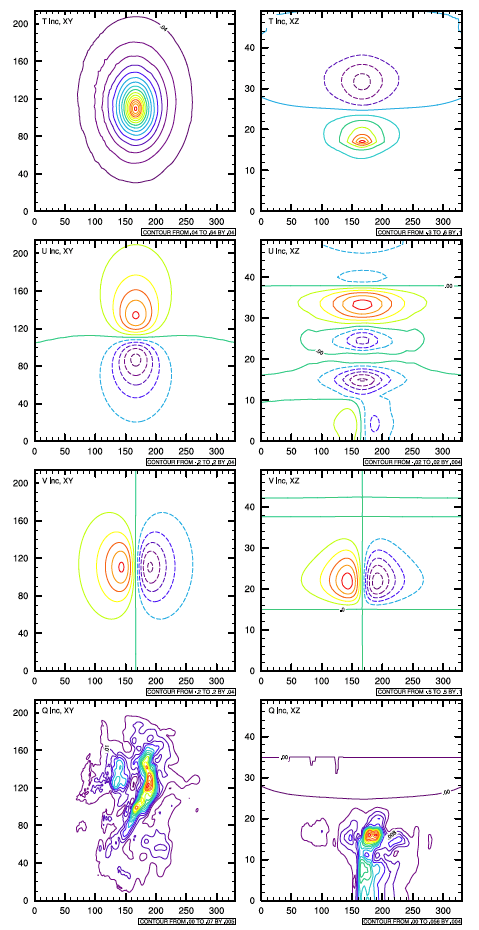
\includegraphics[width=0.7\textwidth]{images/SingleObs}
  \caption{Horizontal cross sections (left column) and vertical cross sections (right column) of analysis increment of T, U, V, and Q from a single T observation}
  \label{fig:singleobs}
\end{figure}

This single observation was located at the center of the domain. The results are shown with figures of the horizontal and vertical cross sections through the point of maximum analysis increment. The Figure \ref{fig:singleobs} was generated using NCL scripts, which can be found in the \textit{util/Analysis\_Utilities/plots\_ncl} directory, introduced in Section A.4.

%-------------------------------------------------------------------------------
\section{Control Data Usage}
\label{sec4.3}
%-------------------------------------------------------------------------------

Observation data used in the GSI analysis can be controlled through three parts of the GSI system:

\begin{enumerate}
\item In the GSI run script, by linking observation BUFR files to the working directory 
\item In section \verb|&OBS_INPUT| of the GSI namelist (inside \textit{comgsi\_namelist.sh})
\item Through parameters in info files (e.g.: convinfo, satinfo, etc.)
\end{enumerate}

Each part provides different levels of control for data usage in the GSI, which is introduced below:

\begin{enumerate}[leftmargin=*]
\item Link observation BUFR files to the working directory in the GSI run script:\\

All BUFR/PrepBUFR observation files need to be linked to the working directory with GSI recognizable names before they can be used in a GSI analysis. The run script (\textit{run\_gsi\_regional.ksh}) makes these links after locating the working directory. Turning these links on or off can control the use of all the data contained in the BUFR files. Table \ref{tab41} provides a list of all default observation file names recognized by GSI and the corresponding examples of the observation BUFR files from NCEP. The following is the first three rows of the table as an example:
\begin{table}[htbp]
\centering
\caption{List of all default observation file names recognized by GSI.}
\begin{tabular}{|p{2cm}|p{9cm}|p{5cm}|}
\hline
\hline
GSI Name & Content & Example file names \\
\hline
prepbufr & Conventional observations, including ps, t, q, pw, uv, spd, dw, sst, from observation platforms such as METAR, soundings, etc. & \textit{gdas1.t12z.prepbufr} \\
\hline
satwndbufr & satellite winds &	\textit{gdas1.t12z.satwnd.tm00.bufr\_d} \\
\hline
amsuabufr & AMSU-A 1b radiance (brightness temperatures) from satellites NOAA-15, 16, 17,18, 19, and METOP-A/B &	\textit{gdas1.t12z.1bamua.tm00.bufr\_d} \\
\hline
\end{tabular}
\label{tab41}
\end{table} 

The left column is the GSI recognized name (bold) and the right column are names of BUFR files from NCEP (italic). In the run script, the following lines are used to link the BUFR files in the right column to the working directory using the GSI recognized names shown in the left column:

\begin{scriptsize}
\begin{verbatim}
# Link to the prepbufr data
ln -s ${PREPBUFR} ./prepbufr

# Link to the radiance data
 ln -s ${OBS_ROOT}/gdas1.t12z.1bamua.tm00.bufr_d amsuabufr
\end{verbatim}
\end{scriptsize}
The GSI recognized default observation filenames are set up in the namelist section \verb|&OBS_INPUT|, which can be changed based on application needs (see below for details). \\

\item In the GSI namelist (inside \textit{comgsi\_namelist.sh}), section \verb|&OBS_INPUT|:\\

In this namelist section, observation files ("dfile" column) are tied to the observation variables used inside the GSI code ("dsis" column). For example, part of section \verb|OBS_INPUT| shows:

\begin{scriptsize}
\begin{verbatim}

&OBS_INPUT
   dmesh(1)=120.0,dmesh(2)=60.0,dmesh(3)=30,time_window_max=1.5,ext_sonde=.true.,
 /
OBS_INPUT::
!  dfile          dtype       dplat     dsis                 dval    dthin dsfcalc
   prepbufr       ps          null      ps                   1.0     0     0
   prepbufr       t           null      t                    1.0     0     0
   prepbufr       q           null      q                    1.0     0     0
   prepbufr       pw          null      pw                   1.0     0     0
   satwndbufr     uv          null      uv                   1.0     0     0
   prepbufr       uv          null      uv                   1.0     0     0
   prepbufr       spd         null      spd                  1.0     0     0
   prepbufr       dw          null      dw                   1.0     0     0
   radarbufr      rw          null      rw                   1.0     0     0
   prepbufr       sst         null      sst                  1.0     0     0
   gpsrobufr      gps_ref     null      gps                  1.0     0     0
   ssmirrbufr     pcp_ssmi    dmsp      pcp_ssmi             1.0    -1     0
   ...
   amsuabufr      amsua       n15       amsua_n15           10.0     2     0
   amsuabufr      amsua       n18       amsua_n18           10.0     2     0
   ...
\end{verbatim}
\end{scriptsize}

This setup tells GSI that conventional observation variables \verb|ps|, \verb|t|, and \verb|q| should be read in from the file prepbufr, while AMSU-A radiances from NOAA-15 and NOAA-18 satellites should be read in from the file \textbf{amsuabufr}. Deleting a particular line in \verb|&OBS_INPUT| will turn off the use of the observation variable presented by the line in the GSI analysis but other variables under the same type can still be used. For example, if we delete: 

\begin{scriptsize}
\begin{verbatim}
amsuabufr      amsua       n15       amsua_n15           10.0     2     0
\end{verbatim}
\end{scriptsize}

Then, the AMSU-A observation from NOAA-15 will not be used in the analysis but the AMSU-A observations from NOAA-18 will still be used.\\


The observation filename in "dfile" can be different from the sample script (\textit{comgsi\_namelist.ksh}). If the filename in "dfile" has been changed, the link from the BUFR files to the GSI recognized name in the run script also needs to be changed correspondingly. For example, if we change the "dfile" in \textbf{amsuabufr} for NOAA-15 to be \verb|amsuabufr_n15|,

\begin{scriptsize}
\begin{verbatim}
amsuabufr_n15    amsua       n15       amsua_n15           10.0     2     0
amsuabufr        amsua       n18       amsua_n18           10.0     2     0
\end{verbatim}
\end{scriptsize}

Then a new link needs to be added in the run script:

\begin{scriptsize}
\begin{verbatim}
# Link to the radiance data
ln -s ${OBS_ROOT}/le_gdas1.t00z.1bamua.tm00.bufr_d amsuabufr
ln -s ${OBS_ROOT}/le_gdas1.t00z.1bamua.tm00.bufr_d amsuabufr_n15
\end{verbatim}
\end{scriptsize}

The GSI will read NOAA-18 AMSU-A observations from file \textbf{amsuabufr} and NOAA-15 AMSU-A observations from file \verb|amsuabufr_n15| based on the above changes to the run scripts and namelist. In this example, both \textbf{amsuabufr} and \verb|amsuabufr_15| are linked to the same BUFR file and NOAA-15 AMSU-A and NOAA-18 AMSU-A observations are still read in from the same BUFR file. If \textbf{amsuabufr} and \verb|amsuabufr_15| link to different BUFR files, then NOAA-15 AMSU-A and NOAA-18 AMSU-A will be read in from different BUFR files. The changeable filename in \textit{dfile} gives GSI more flexibility to handle multiple data resources.\\


\item Use info files to control data usage\\

For each variable, observations can come from multiple platforms (data types or observation instruments). For example, surface pressure (ps) can come from METAR observation stations (data type 187) and rawinsonde (data type 120). There are several files named *info in the GSI system (located in \textit{./fix}) to control the usage of observations based on the observation platform. Table \ref{tab42} is a list of info files and their function:
\begin{table}[htbp]
\centering
\caption{The content of info files }
\begin{tabular}{|p{2cm}|p{14cm}|}
\hline
\hline
File name in GSI & Function and Content \\
\hline
convinfo & Control the usage of conventional data, including tcp, ps, t, q, pw, sst, uv, spd, dw, radial wind (Level 2 \textit{rw} and 2.5 \textit{srw}), gps, and \textit{pm2\_5} \\
\hline
satinfo	 & Control the usage of satellite data. Instruments include AMSU-A/B, HIRS3/4, MHS, ssmi, ssmis, iasi, airs, sndr, cris, amsre, imgr, seviri, atms, avhrr3, etc., and satellites include NOAA 15, 17, 18, 19, aqua, GOES 11, 12, 13, METOP-A/B, NPP, DMSP 15,16,17,18,19,20, 
M08, M09, M10, etc.\\
ozinfo & Control the usage of ozone data, including sbuv6, 8 from NOAA 14, 16, 17, 18, 19. omi\_aura, gome\_metop-a, and mls\_aura \\
\hline
pcpinfo	& Control the usage of precipitation data, including pcp\_ssmi and pcp\_tmi \\
\hline
aeroinfo & Control the usage of aerosol data, including modis\_aqua and modis\_terra \\
\hline
\end{tabular}
\label{tab42}
\end{table} 

The header of each info file includes an explanation of the content of the file. Here we discuss the two most commonly used info files:

\begin{itemize}[leftmargin=*]
\item convinfo\\

The \textbf{convinfo} file controls the usage of conventional data. The following is part of the \textbf{convinfo} file:

\begin{tiny}
\begin{verbatim}

!otype   type  sub iuse twindow numgrp ngroup nmiter gross ermax ermin var_b    var_pg ithin rmesh  pmesh  npred  pmot  ptime
 tcp      112    0    1     3.0      0      0      0  75.0   5.0   1.0  75.0  0.000000     0    0.     0.      0    0.     0.
 ps       120    0    1     3.0      0      0      0   4.0   3.0   1.0   4.0  0.000300     0    0.     0.      0    0.     0.
 ps       132    0   -1     3.0      0      0      0   4.0   3.0   1.0   4.0  0.000300     0    0.     0.      0    0.     0.
 ps       180    0    1     3.0      0      0      0   4.0   3.0   1.0   4.0  0.000300     0    0.     0.      0    0.     0.
 ps       180    01   1     3.0      0      0      0   4.0   3.0   1.0   4.0  0.000300     0    0.     0.      0    0.     0.
 ps       181    0    1     3.0      0      0      0   3.6   3.0   1.0   3.6  0.000300     0    0.     0.      0    0.     0.
 ps       182    0    1     3.0      0      0      0   4.0   3.0   1.0   4.0  0.000300     0    0.     0.      0    0.     0.
 ps       183    0   -1     3.0      0      0      0   4.0   3.0   1.0   4.0  0.000300     0    0.     0.      0    0.     0.
 ps       187    0    1     3.0      0      0      0   4.0   3.0   1.0   4.0  0.000300     0    0.     0.      0    0.     0.
 t        120    0    1     3.0      0      0      0   8.0   5.6   1.3   8.0  0.000001     0    0.     0.      0    0.     0.
 t        126    0   -1     3.0      0      0      0   8.0   5.6   1.3   8.0  0.001000     0    0.     0.      0    0.     0.
 t        130    0    1     3.0      0      0      0   7.0   5.6   1.3   7.0  0.001000     0    0.     0.      0    0.     0.
 t        131    0    1     3.0      0      0      0   7.0   5.6   1.3   7.0  0.001000     0    0.     0.      0    0.     0.
 t        132    0    1     3.0      0      0      0   7.0   5.6   1.3   7.0  0.001000     0    0.     0.      0    0.     0.
 t        133    0    1     3.0      0      0      0   7.0   5.6   1.3   7.0  0.004000     0    0.     0.      0    0.     0.
 t        134    0   -1     3.0      0      0      0   7.0   5.6   1.3   7.0  0.004000     0    0.     0.      0    0.     0.
 t        135    0   -1     3.0      0      0      0   7.0   5.6   1.3   7.0  0.004000     0    0.     0.      0    0.     0.
 t        180    0    1     3.0      0      0      0   7.0   5.6   1.3   7.0  0.004000     0    0.     0.      0    0.     0.
 t        180    01   1     3.0      0      0      0   7.0   5.6   1.3   7.0  0.004000     0    0.     0.      0    0.     0.
 t        181    0   -1     3.0      0      0      0   7.0   5.6   1.3   7.0  0.004000     0    0.     0.      0    0.     0.
 t        182    0    1     3.0      0      0      0   7.0   5.6   1.3   7.0  0.004000     0    0.     0.      0    0.     0.
\end{verbatim}
\end{tiny}

The meaning of each column is explained in the header of the file and is listed in Table \ref{tab43}. \\

\begin{table}[htbp]
\centering
\caption{list of the content for each convinfo column}
\begin{tabular}{|p{2cm}|p{14cm}|}
\hline
\hline
Column Name & Content of the column \\
\hline
otype & observation variables (t, uv, q, etc.) \\
\hline
type & prepbufr observation type (if available) \\
\hline
sub	& prepbufr subtype (not yet available) \\
\hline
iuse & flag if to use/not use / monitor data; \newline
= 1, use data, the data type will be read and used in the analysis after quality control;\newline
= 0, read in and process data, use for quality control, but do NOT assimilate;\newline
= -1, monitor data. This data type will be read in and monitored but not be used in the GSI analysis. \\
\hline
twindow	& time window (+/- hours) for data used in the analysis \\
\hline
numgrp & cross validation parameter - number of groups \\
\hline
ngroup & cross validation parameter - group to remove from data use \\
\hline
nmiter & cross validation parameter - external iteration to introduce removed data \\
\hline
gross & gross error parameter - gross error \\
\hline
ermax & gross error parameter - maximum error \\
\hline
ermin & gross error parameter - minimum error \\
\hline
var\_b & variational quality control parameter - b parameter \\
\hline
var\_pg & variational quality control parameter - pg parameter\\
\hline
ithin & Flag to turn on thinning (0, no thinning, 1 - thinning) \\
\hline
rmesh & size of horizontal thinning mesh (in kilometers) \\
\hline
pmesh & size of vertical thinning mesh \\
\hline
npred & Number of bias correction predictors \\
\hline
pmot & Option to keep thinned data as monitored, 0: do not keep, other values: keep \\
\hline
ptime & time interval for thinning, 0, no temporal thinning, other values define time interval (less than six) \\
\hline
\end{tabular}
\label{tab43}
\end{table} 

From this table, we can see that parameter "iuse" is used to control the usage of data and parameter "twindow" is used to control the time window of data usage. Parameters gross, ermax, and ermin are for gross quality control. Through these parameters, GSI can control how to use certain types of data in the analysis.\\

\item satinfo\\

The \textit{satinfo} file contains information about the channels, sensors, and satellites.  It specifies observation error (cloudy or clear) for each channel, how to use the channels (assimilate, monitor, etc), and other useful information. The following is part of the content of \textit{satinfo}. The meaning of each column is explained in Table \ref{tab44}.

\begin{scriptsize}
\begin{verbatim}

!sensor/instr/sat      chan iuse  error  error_cld  ermax   var_b    var_pg  cld_det
 amsua_n15               1   1    3.000   20.000    4.500   10.000    0.000     -2
 amsua_n15               2   1    2.200   18.000    4.500   10.000    0.000     -2
 amsua_n15               3   1    2.000   12.000    4.500   10.000    0.000     -2
 amsua_n15               4   1    0.600    3.000    2.500   10.000    0.000     -2
 amsua_n15               5   1    0.300    0.500    2.000   10.000    0.000     -2
 amsua_n15               6  -1    0.230    0.300    2.000   10.000    0.000     -2
 amsua_n15               7   1    0.250    0.250    2.000   10.000    0.000     -2
 amsua_n15               8   1    0.275    0.275    2.000   10.000    0.000     -2
 amsua_n15               9   1    0.340    0.340    2.000   10.000    0.000     -2
 amsua_n15              10   1    0.400    0.400    2.000   10.000    0.000     -2
 amsua_n15              11  -1    0.600    0.600    2.500   10.000    0.000     -2
 amsua_n15              12   1    1.000    1.000    3.500   10.000    0.000     -2
 amsua_n15              13   1    1.500    1.500    4.500   10.000    0.000     -2
 amsua_n15              14  -1    2.000    2.000    4.500   10.000    0.000     -2
 amsua_n15              15   1    3.500   15.000    4.500   10.000    0.000     -2
 hirs3_n17               1  -1    2.000    0.000    4.500   10.000    0.000     -1
 hirs3_n17               2  -1    0.600    0.000    2.500   10.000    0.000      1
 hirs3_n17               3  -1    0.530    0.000    2.500   10.000    0.000      1
\end{verbatim}
\end{scriptsize}

\begin{table}[htbp]
\centering
\caption{list of the content for each satinfo column}
\begin{tabular}{|p{4cm}|p{10cm}|}
\hline
\hline
Column Name & Content of the column \\
\hline
\hline
sensor/instr/sat & Sensor, instrument, and satellite name \\
\hline
chan & Channel number for certain sensor\\
\hline
iuse& = 1, use this channel data; \newline
=-1, don\textquotesingle t use this channel data \\
\hline
error	& Variance for each satellite channel \\
\hline
error\_cld & Variance for each satellite channel if cloudy \\
\hline
ermax & Error maximum for gross check to observations \\
\hline
var\_b & Possible range of variable for gross errors \\
\hline
var\_pg  & Probability of gross error \\
\hline
icld\_det  & Use this channel in cloud detection if > 0 \\
\hline
\end{tabular}
\label{tab44}
\end{table} 


\end{itemize}
 
\end{enumerate}

%-------------------------------------------------------------------------------
\section{Domain Partition for Parallelization and Observation Distribution}
\label{sec4.4}
%-------------------------------------------------------------------------------

The standard output file (\textit{stdout}) has an information block that shows the distribution of different kinds of observations in each sub-domain. This block follows the observation input section. The following is the observation distribution from the case shown in Section \ref{sec4.1}. From the introduction, we know the prepbufr (conventional data), radiance BUFR files, and GPS BUFR files were used. In this list, the conventional observations (\verb|ps|, \verb|t|, \verb|q|, \verb|pw|, and \verb|uv|), GPSRO (\verb|gps_ref|), and radiance data (\verb|amusa|, \verb|hirs4|, and \verb|mhs| from \verb|Metop-a|, \verb|Metop-b|, \verb|NOAA 15|, and \verb|18|) were distributed among four sub-domains:

\begin{scriptsize}
\begin{verbatim}
OBS_PARA: ps                        1429      3190      4655      6774
OBS_PARA: t                         2564      5200      7057     11128
OBS_PARA: q                         2346      4626      6148      8128
OBS_PARA: pw                          65        80        63        49
OBS_PARA: uv                        3358      6453      8091     11998
OBS_PARA: gps_ref                   1799      1368      2664      3520
OBS_PARA: hirs4     metop-a            0         0      1146      1661
OBS_PARA: hirs4     n19              213      1020         0         0
OBS_PARA: hirs4     metop-b            0         0        85       555
OBS_PARA: amsua     n15             1458      2026       830       234
OBS_PARA: amsua     n18             2223      2318       108         0
OBS_PARA: amsua     n19              176       960         0         0
OBS_PARA: amsua     metop-a            0         0      1077      1559
OBS_PARA: amsua     metop-b            0         0       265      1829
OBS_PARA: mhs       n18             2550      2695       160         0
OBS_PARA: mhs       n19              246      1103         0         0
OBS_PARA: mhs       metop-a            0         0      1237      1809
OBS_PARA: mhs       metop-b            0         0       321      2128
\end{verbatim}
\end{scriptsize}

This list is a good way to quickly check which kinds of data are used in the analysis and how they are distributed in the analysis domain.


%-------------------------------------------------------------------------------
\section{Observation Innovation Statistics}
%-------------------------------------------------------------------------------

The GSI analysis provides a set of files named \textit{fort.2*} to summarize observations fit to the current solution in each outer loop (except for \textit{fort.220}, see explanation in the next section). The content of some of these files is listed in Table \ref{tab45}:

\begin{table}[htbp]
\centering
\caption{List of the content and units for each fort files}
\begin{tabular}{|p{4cm}|p{7cm}|p{3cm}|}
\hline
\hline
File Name & Variables in file & Ranges/units \\
\hline
\textit{fort.201 or fit\_p1.analysis\_time} & fit of surface pressure data & mb \\
\hline
\textit{fort.202 or fit\_w1.analysis\_time} & fit of u, v wind data & m/s \\
\hline
\textit{fort.203 or fit\_t1.analysis\_time} & fit of temperature data & K \\
\hline
\textit{fort.204 or fit\_q1.analysis\_time} & fit of moisture data & percent of qsaturation guess \\
\hline
\textit{fort.205} & fit of precipitation water data & mm \\
\hline
\textit{fort.206} & fit of ozone observations from sbuv6\_n14 (, \_n16, \_n17, \_n18), sbuv8\_n16 (, \_n17, \_n18, \_n19), omi\_aura, gome\_metop-a/b, and mls\_aura &  \\
\hline
\textit{fort.207 or fit\_rad1.analysis\_time} & fit of satellite radiance data, such as:
amsua\_n15(, n16, n17, n18, metop-a, aqua, n19), amsub\_n17, hirs3\_n17, hirs4\_n19 (, metop-a), etc. & \\
\hline	
\textit{fort.208} & fit of precipitation rate (pcp\_ssmi and pcp\_tmi) & \\	
\hline
\textit{fort.209} & fit of radar radial wind (rw) & \\
\hline
\textit{fort.210} & fit of lidar wind (dw) & \\
\hline
\textit{fort.211} & fit of radar superob wind data (srw) & \\
\hline	
\textit{fort.212} & fit of GPS data (refractivity or bending angle) & fractional difference \\
\hline
\textit{fort.213} & fit of conventional sst data & C \\
\hline
\textit{fort.214} & fit of tropical cyclone central pressure &  \\
\hline
\textit{fort.215} & fit of Lagrangian tracer data &  \\
\hline
\textit{fort.217} & fit of aerosol product (aod) &  \\
\hline	
\textit{fort.218} & fit of wind gust &  \\
\hline	
\textit{Fort.219} & fit of visibility &
 \\
\hline
\end{tabular}
\label{tab45}
\end{table} 

To help users understand the information inside these files, some examples are given in the following sub-sections with corresponding explanations.

%-------------------------------------------------------------------------------
\subsection{Conventional observations}
\label{sec4.5.1}
%-------------------------------------------------------------------------------

Example of files, including single level data (\textit{fort.201}, \textit{fort.205}, and \textit{fort.213})

\begin{scriptsize}
\begin{verbatim}
current fit of surface pressure data, ranges in mb
--------------------------------------------------
 pressure levels (hPa)=   0.0 2000.0
     it     obs    type stype    count      bias       rms      cpen     qcpen
 o-g 01      ps     120 0000       101    0.1813    0.6089    0.4711    0.4711
 o-g 01      ps     180 0000       601    0.0378    0.6354    0.7171    0.7171
 o-g 01      ps     180 0001      1428    0.1857    0.8555    0.7164    0.7164
 o-g 01      ps     181 0000       610    0.1959    0.8991    0.7387    0.7387
 o-g 01      ps     182 0000         1    0.9173    0.9173    2.8976    2.8976
 o-g 01      ps     187 0000     11149    0.1999    0.7877    0.3360    0.3360
 o-g 01             all          13890    0.1912    0.7931    0.4105    0.4105
 o-g 01      ps rej 120 0000         1   -3.5799    3.5799    0.0000    0.0000
 o-g 01      ps rej 180 0001         7   -0.3349    4.9273    0.0000    0.0000
 o-g 01      ps rej 181 0000        47    1.1146   54.8539    0.0000    0.0000
 o-g 01      ps rej 183 0000         3   10.4797   10.4836    0.0000    0.0000
 o-g 01      ps rej 187 0000        52    4.2528    7.4112    0.0000    0.0000
 o-g 01         rej all            110    2.7186   36.2804    0.0000    0.0000
 o-g 01      ps mon 132 0000         1    0.9173    0.9173    0.2104    0.2104
 o-g 01      ps mon 180 0000       113    0.0447    0.5158    0.8709    0.8709
 o-g 01      ps mon 180 0001        24    0.2122    0.4050    0.3559    0.3559
 o-g 01      ps mon 181 0000       207    0.0910    0.9492    1.2514    1.2514
 o-g 01      ps mon 183 0000      1386    0.3974    1.0861    0.0000    0.0000
 o-g 01      ps mon 187 0000        88   -0.0100    0.5290    0.7534    0.7534
 o-g 01         mon all           1819    0.3188    1.0169    0.2378    0.2378
\end{verbatim}
\end{scriptsize}

Example of files including multiple level data (\textit{fort.202}, \textit{fort.203}, and \textit{fort.204})

\begin{scriptsize}
\begin{verbatim}
                              ptop  1000.0  900.0  800.0  600.0  100.0   50.0     0.0
     it     obs    type styp  pbot  1200.0 1000.0  900.0  800.0  150.0  100.0  2000.0
------------------------------------------------------------------------------------------
 o-g 01      uv     220 0000 count      44    223    223    478    437    519    4231
 o-g 01      uv     220 0000  bias    0.26   0.51   0.04   0.35   0.99   0.97    0.59
 o-g 01      uv     220 0000   rms    2.21   2.48   2.51   2.84   5.88   4.79    4.18
 o-g 01      uv     220 0000  cpen    0.31   0.38   0.44   0.61   1.64   1.18    0.90
 o-g 01      uv     220 0000 qcpen    0.31   0.38   0.44   0.60   1.63   1.18    0.89
 o-g 01      uv     223 0000 count       0      6     16     88     32      8     331
 o-g 01      uv     223 0000  bias    0.00   0.23  -0.29   0.85  -0.76  -4.89    0.27
 o-g 01      uv     223 0000   rms    0.00   1.28   1.32   2.86   5.21   6.63    3.76
 o-g 01      uv     223 0000  cpen    0.00   0.06   0.07   0.45   0.88   1.31    0.73

...
 
 o-g 01             all      count    1799   1726   2001   3050    469    527   13124
 o-g 01             all       bias    0.05   0.91   0.78   0.63   0.87   0.88    0.62
 o-g 01             all        rms    2.46   2.58   2.65   3.21   5.83   4.82    3.54
 o-g 01             all       cpen    0.24   0.24   0.30   0.45   1.58   1.19    0.52
 o-g 01             all      qcpen    0.23   0.24   0.30   0.44   1.58   1.19    0.52
 o-g 01      uv rej 220 0000 count       0      0      0      0      0      0     800
 o-g 01      uv rej 220 0000  bias    0.00   0.00   0.00   0.00   0.00   0.00    3.11
 o-g 01      uv rej 220 0000   rms    0.00   0.00   0.00   0.00   0.00   0.00    6.41

...

 o-g 01         rej all      count      23    108     21     41     2      0    1008
 o-g 01         rej all       bias   44.72   6.40  -0.30  -7.38  11.46   0.00    3.84
 o-g 01         rej all        rms   56.08  16.60   6.87  10.47  43.15   0.00   12.28
 o-g 01         rej all       cpen    0.00   0.00   0.00   0.00   0.00   0.00    0.00
 o-g 01         rej all      qcpen    0.00   0.00   0.00   0.00   0.00   0.00    0.00
 o-g 01      uv mon 220 0000 count       0      4      0      1      8      9      29
 o-g 01      uv mon 220 0000  bias    0.00   1.07   0.00   6.04  -1.03   0.23   -2.21
 o-g 01      uv mon 220 0000   rms    0.00  20.49   0.00  17.78   9.06   8.51   12.52
 o-g 01      uv mon 220 0000  cpen    0.00   0.00   0.00   0.00   0.00   0.00    0.00
 o-g 01      uv mon 220 0000 qcpen    0.00   0.00   0.00   0.00   0.00   0.00    0.00

...
 
 o-g 01         mon all      count    3573   7736   1004    563      8      9   13052
 o-g 01         mon all       bias   -0.01   0.40   0.05  -0.30  -1.03   0.23    0.23
 o-g 01         mon all        rms    2.55   3.25   4.67   5.98   9.06   8.51    3.60
 o-g 01         mon all       cpen    0.81   1.21   1.67   1.28   0.00   0.00    1.12
 o-g 01         mon all      qcpen    0.80   1.15   1.53   1.16   0.00   0.00    1.07
...
\end{verbatim}
\end{scriptsize}

Please note that five layers from 600 to 150 hPa have been deleted to make each row fit into one line. Only observation type 220 and 223 are shown as an example.

Table \ref{tab46} lists the meaning of each item in file \textit{fort.201-213} except file \textit{fort.207}:

\begin{table}[htbp]
\centering
\caption{List of each item in file fort.201-213 (except fort.207).}
\begin{tabular}{|p{1cm}|p{10cm}|}
\hline
\hline
 Name & Explanation \\
\hline
\textit{it} & outer loop number \newline
= 01: observation - background \newline
= 02: observation - analysis (after 1\textsuperscript{st} outer loop) \newline
= 03: observation - analysis (after 2\textsuperscript{nd} outer loop) \\
\hline
\textit{obs} & observation variable type (such as uv or ps) and usage, which includes: \newline
blank: used in GSI analysis \newline
mon: monitored (read in but not assimilated by GSI) \newline
rej: rejected because of quality control in GSI \\
\hline
\textit{type} & prepbufr observation type (see the BUFR User\textquotesingle s Guide for details) \\
\hline
\textit{styp} & prepbufr observation subtype (not used) \\
\hline
\textit{ptop} & for multiple level data: pressure at the top of the layer \\
\hline
\textit{pbot} & for multiple level data: pressure at the bottom of the layer \\
\hline
\textit{count} & the number of observations summarized under observation types and vertical layers  \\
\hline
\textit{bias} & bias of observation departure for each outer loop (it) \\
\hline
\textit{rms} & root mean square error of observation departure for each outer loop (it)  \\
\hline
\textit{cpen} & observation part of penalty (cost function) \\
\hline
\textit{qcpen} & nonlinear qc penalty \\
\hline
\end{tabular}
\label{tab46}
\end{table} 

The contents of the fit files are calculated based on O-B or O-A for each observation. The detailed departure information about each observation is saved in the diagnostic files. For the content of the diagnostic files, please check the content of the array "rdiagbuf" in one of the setup subroutines for conventional data (for example, setupt.f90). We provide a tool in appendix A.2 to help users read in the information from the diagnostic files.

These fit files give lots of useful information on how data are analyzed by the GSI, such as how many observations are used and rejected, the bias and root mean squared (RMS) error for certain data types or for all observations, and how analysis results fit to the observation before and after analysis. Again, we use observation type 220 in \textit{fort.202} (\textit{fit\_w1.2014061700}) as an example to illustrate how to read this information. The fit information for observation type 220 (soundings) is listed below. Like the previous example, five layers from 600 to 150 hPa were deleted to make each row fit into one line. All fit information of observation type 220 is shown. 

\begin{scriptsize}
\begin{verbatim}
                              ptop  1000.0  900.0  800.0  600.0  100.0   50.0     0.0
     it     obs    type styp  pbot  1200.0 1000.0  900.0  800.0  150.0  100.0  2000.0
-------------------------------------------------------------------------------------
 o-g 01      uv     220 0000 count      44    223    223    478    437    519    4231
 o-g 01      uv     220 0000  bias    0.26   0.51   0.04   0.35   0.99   0.97    0.59
 o-g 01      uv     220 0000   rms    2.21   2.48   2.51   2.84   5.88   4.79    4.18
 o-g 01      uv     220 0000  cpen    0.31   0.38   0.44   0.61   1.64   1.18    0.90
 o-g 01      uv     220 0000 qcpen    0.31   0.38   0.44   0.60   1.63   1.18    0.89

...
 o-g 01      uv rej 220 0000 count       0      0      0      0      0      0     800
 o-g 01      uv rej 220 0000  bias    0.00   0.00   0.00   0.00   0.00   0.00    3.11
 o-g 01      uv rej 220 0000   rms    0.00   0.00   0.00   0.00   0.00   0.00    6.41
 o-g 01      uv rej 220 0000  cpen    0.00   0.00   0.00   0.00   0.00   0.00    0.00
 o-g 01      uv rej 220 0000 qcpen    0.00   0.00   0.00   0.00   0.00   0.00    0.00

...

 o-g 01      uv mon 220 0000 count       0      4      0      1      8      9      29
 o-g 01      uv mon 220 0000  bias    0.00   1.07   0.00   6.04  -1.03   0.23   -2.21
 o-g 01      uv mon 220 0000   rms    0.00  20.49   0.00  17.78   9.06   8.51   12.52
 o-g 01      uv mon 220 0000  cpen    0.00   0.00   0.00   0.00   0.00   0.00    0.00
 o-g 01      uv mon 220 0000 qcpen    0.00   0.00   0.00   0.00   0.00   0.00    0.00

...

                              ptop  1000.0  900.0  800.0  600.0  100.0   50.0     0.0
     it     obs    type styp  pbot  1200.0 1000.0  900.0  800.0  150.0  100.0  2000.0
-------------------------------------------------------------------------------------
 o-g 02      uv     220 0000 count      44    223    223    478    437    519    4231
 o-g 02      uv     220 0000  bias    0.21   0.05  -0.43   0.03   0.69   0.96    0.39
 o-g 02      uv     220 0000   rms    2.13   2.26   2.29   2.56   5.19   4.55    3.73
 o-g 02      uv     220 0000  cpen    0.32   0.31   0.37   0.50   1.27   1.07    0.71
 o-g 02      uv     220 0000 qcpen    0.32   0.31   0.37   0.50   1.27   1.07    0.71

...

 o-g 02      uv rej 220 0000 count       0      0      0      0      0      0     800
 o-g 02      uv rej 220 0000  bias    0.00   0.00   0.00   0.00   0.00   0.00    2.96
 o-g 02      uv rej 220 0000   rms    0.00   0.00   0.00   0.00   0.00   0.00    6.33
 o-g 02      uv rej 220 0000  cpen    0.00   0.00   0.00   0.00   0.00   0.00    0.00
 o-g 02      uv rej 220 0000 qcpen    0.00   0.00   0.00   0.00   0.00   0.00    0.00

...

 o-g 02      uv mon 220 0000 count       0      4      0      1      8      9      29
 o-g 02      uv mon 220 0000  bias    0.00   2.16   0.00   5.80  -1.00   0.23   -0.82
 o-g 02      uv mon 220 0000   rms    0.00  18.44   0.00  12.60  10.31   8.58   10.87
 o-g 02      uv mon 220 0000  cpen    0.00   0.00   0.00   0.00   0.00   0.00    0.00
 o-g 02      uv mon 220 0000 qcpen    0.00   0.00   0.00   0.00   0.00   0.00    0.00


...
                              ptop  1000.0  900.0  800.0  600.0  100.0   50.0     0.0
     it     obs    type styp  pbot  1200.0 1000.0  900.0  800.0  150.0  100.0  2000.0
----------------------------------------------------------------------------------------
 o-g 03      uv     220 0000 count      44    223    223    478    437    519    4231
 o-g 03      uv     220 0000  bias    0.28   0.08  -0.32   0.11   0.74   1.00    0.43
 o-g 03      uv     220 0000   rms    2.11   2.17   2.20   2.38   5.00   4.46    3.60
 o-g 03      uv     220 0000  cpen    0.31   0.29   0.34   0.43   1.18   1.03    0.65
 o-g 03      uv     220 0000 qcpen    0.31   0.29   0.34   0.43   1.18   1.03    0.65

...

 o-g 03      uv rej 220 0000 count       0      0      0      0      0      0     800
 o-g 03      uv rej 220 0000  bias    0.00   0.00   0.00   0.00   0.00   0.00    2.98
 o-g 03      uv rej 220 0000   rms    0.00   0.00   0.00   0.00   0.00   0.00    6.35
 o-g 03      uv rej 220 0000  cpen    0.00   0.00   0.00   0.00   0.00   0.00    0.00
 o-g 03      uv rej 220 0000 qcpen    0.00   0.00   0.00   0.00   0.00   0.00    0.00

...

 o-g 03      uv mon 220 0000 count       0      4      0      1      8      9      29
 o-g 03      uv mon 220 0000  bias    0.00   1.86   0.00   6.09  -0.98   0.07   -0.94
 o-g 03      uv mon 220 0000   rms    0.00  18.76   0.00  12.59  10.34   8.69   11.01
 o-g 03      uv mon 220 0000  cpen    0.00   0.00   0.00   0.00   0.00   0.00    0.00
 o-g 03      uv mon 220 0000 qcpen    0.00   0.00   0.00   0.00   0.00   0.00    0.00

\end{verbatim}
\end{scriptsize}

In loop section \verb|o-g 01|, from the \verb|count| line, we can see there were 4231 sounding observations used in the analysis. Among them, 44 were within the 1000-1200 hPa layer. Also from the \verb|count| lines, in the rejection and monitoring section, there were 800 observations rejected and 29 observations monitored. In the same loop section, from the \verb|bias| line and \verb|rms| lines, we can see the total bias and RMS error of O-B for the sounding information is 0.59 and 4.18. The bias and RMS error for each vertical layer can also be found in this file.

Next we can see bias and RMS error values from different loops, as shown with the comparison in the following three lines:

\begin{scriptsize}
\begin{verbatim}
o-g 01      uv     220 0000   rms    2.21   2.48   2.51   2.84   5.88   4.79    4.18
o-g 02      uv     220 0000   rms    2.13   2.26   2.29   2.56   5.19   4.55    3.73
o-g 03      uv     220 0000   rms    2.11   2.17   2.20   2.38   5.00   4.46    3.60
\end{verbatim}
\end{scriptsize}

These three lines show that the RMS error reduced from 4.18 (o-g 01, which is O-B) to 3.73 (o-g 02, which is O-A after the 1\textsuperscript{st} outer loop) and then to 3.60 (o-g 03, which is O-A after the 2\textsuperscript{nd} outer loop, which is also the final analysis result). The reduction in the RMS error shows that observation type 220 (sounding) was used in the GSI analysis to modify the background fields to fit to the observations. 

%-------------------------------------------------------------------------------
\subsection{Satellite Radiance}
\label{sec4.5.2}
%-------------------------------------------------------------------------------

The file \textit{fort.207} is the fit file for radiance data. Its content includes important information about the radiance data analysis.

The first part of the file \textit{fort.207} lists the content that corresponds to those in the file \textbf{satinfo}, which is the info file to control radiance data usage. 

\begin{tiny}
\begin{verbatim}

RADINFO_READ:  jpch_rad=   2723
   1 amsua_n15            chan=    1 var=   3.000 varch_cld= 20.000 use=  1 ermax=   4.500 b_rad=   10.00 pg_rad=   0.00 icld_det=-2
   2 amsua_n15            chan=    2 var=   2.200 varch_cld= 18.000 use=  1 ermax=   4.500 b_rad=   10.00 pg_rad=   0.00 icld_det=-2
   3 amsua_n15            chan=    3 var=   2.000 varch_cld= 12.000 use=  1 ermax=   4.500 b_rad=   10.00 pg_rad=   0.00 icld_det=-2
   4 amsua_n15            chan=    4 var=   0.600 varch_cld=  3.000 use=  1 ermax=   2.500 b_rad=   10.00 pg_rad=   0.00 icld_det=-2
   5 amsua_n15            chan=    5 var=   0.300 varch_cld=  0.500 use=  1 ermax=   2.000 b_rad=   10.00 pg_rad=   0.00 icld_det=-2

...
\end{verbatim}
\end{tiny}

This shows there are 2723 channels listed in the \textit{satinfo} file and the 2723 lines following this line include the details for each channel.

The second part of the file is a list of the coefficients for bias correction, after reading the \textit{satbias\_in} file:

\begin{tiny}
\begin{verbatim}
 RADINFO_READ: ***WARNING instrument/channel ahi_himawari8                 16
  not found in satbias_pc file - set to zero
 RADINFO_READ:  guess air mass bias correction coefficients below
   1            amsua_n15   -1.965181    0.000000   39.068176   -0.923195    0.408460    0.000000    0.000000    0.001735    3.689709    
                                    2.367472    8.862940   -1.848292
   2            amsua_n15   -7.415403    0.000000   80.138019   -0.818472   -1.013216    0.000000    0.000000    0.014279    2.638804    
                                    8.315096   22.041458   -1.564773
...
\end{verbatim}
\end{tiny}

Each channel has 12 coefficients listed in a line. Therefore, there are 2723 lines of radiance bias correction coefficients for all channels, though some of the coefficients are zero.

The 3\textsuperscript{rd} part of the \textit{fort.207} file is similar to other fit files with content repeated in three sections, providing detailed statistics about the data in stages before the 1\textsuperscript{st} outer loop, between the 1\textsuperscript{st} and 2\textsuperscript{nd} outer loops, and after the 2\textsuperscript{nd} outer loop. The results before the 1\textsuperscript{st} outer loop are used here as an example to explain the content of the results:

\begin{itemize}[leftmargin=*]

\item Summaries for various statistics as a function of observation type
  
\begin{scriptsize}
\begin{verbatim} 
 sat       type              penalty    nobs   iland isnoice  icoast ireduce   ivarl nlgross
 metop-a    hirs4         371.46818888    385     143       0      25       0    1452       0
                            qcpenalty     qc1     qc2     qc3     qc4     qc5     qc6     qc7
                          371.46818888      0       0    1651    3330       0       0       0


  sat       type              penalty    nobs   iland isnoice  icoast ireduce   ivarl nlgross
 metop-b    hirs4           0.00000000     34      25       0       0       0     139       0
                            qcpenalty     qc1     qc2     qc3     qc4     qc5     qc6     qc7
                            0.00000000      0       0      97     279       0       0       0

      6

rad total   penalty_all=   13986.0933845987129
rad total qcpenalty_all=   13986.0933845987129
rad total failed nonlinqc=                         0

...
\end{verbatim}
\end{scriptsize}

Table \ref{tab47} outlines the meaning of each item in the above statistics:

\begin{table}[htbp]
\centering
\caption{Summary of the radiance observation fit file (fort.207)}
\begin{tabular}{|p{2cm}|p{10cm}|}
\hline
\hline
 Name & Explanation \\
\hline
\hline
\textit{sat} & satellite name \\
\hline
\textit{type} & instrument type \\
\hline
\textit{penalty} & contribution to cost function from this observation type \\
\hline
\textit{nobs} & number of good observations used in the assimilation\\
\hline
\textit{iland} & number of observations over land \\
\hline
\textit{isnoice} & number of observations over sea ice and snow \\
\hline
\textit{icoast} & number of observations over coast  \\
\hline
\textit{ireduce} & number of observations that reduce qc bounds in tropics \\
\hline
\textit{ivarl} & number of observations removed by gross check  \\
\hline
\textit{nlgross} & number of observation removed by nonlinear qc\\
\hline
\textit{qcpenalty} & nonlinear qc penalty from this data type \\
\hline
\textit{qc1-7} & number of observations whose quality control criteria has been adjusted by each qc method (1-7).  For details, see the Radiance Chapter of the Advanced User\textquotesingle s Guide \\
\hline
\textit{rad total penalty\_all} & summary of penalty for all radiance observation types \\
\hline
\textit{rad total qcpenalty\_all} & summary of qcpenalty for all radiance observation types \\
\hline
\textit{rad total failed nonlinqc} & summary of observations removed by nonlinear qc for all radiance observation types \\
\hline
\end{tabular}
\label{tab47}
\end{table} 

Note: One radiance observation may include multiple channels, and not all channels are necessarily used in the analysis.

\item Summaries for various statistics as a function of channel

\begin{scriptsize}
\begin{verbatim}

 1  2    3        4   5       6         7           8         9        10       11
 1  1 amsua_n15  915 247  3.000  0.6623748  1.2673027  0.2414967  2.4209147  2.0627099
 2  2 amsua_n15  902 261  2.000  0.5209886  1.1773765  0.2626527  2.2705374  1.9414234
 3  3 amsua_n15 1114  48  2.000  1.2349467 -1.5090660  0.3421312  1.9416738  1.2218089
 4  4 amsua_n15 1162   0  0.600 -0.2114506 -0.3195250  0.5286580  0.6271317  0.5396275
 5  5 amsua_n15 1162   3  0.300 -0.0888496 -0.1685199  0.4352839  0.2734131  0.2153040
 6  6 amsua_n15 2093   3 -0.230 -1.8141034 -0.0695503  0.8415303  0.2646033  0.2552992
 7  7 amsua_n15 2342  28  0.250 -0.0830293  0.0453835  0.6141132  0.2522587  0.2481427
 8  8 amsua_n15 2311  59  0.275  0.0201868  0.1758359  0.7782391  0.3173862  0.2642267
 9  9 amsua_n15 2124 246  0.340  0.1262987  0.5008846  1.4907547  0.5544190  0.2376868
10 10 amsua_n15   82 2288 0.400  0.6700157  0.8263504  2.0387089  0.8304076  0.0819868
15 15 amsua_n15  862  300 3.000  0.8244923 -2.2960147  0.3769625  2.7445692  1.5036544

...

63  4 hirs4_metop-a  11 217 0.400  0.9717384  0.9536444  1.8583033  0.9570578  0.0807581
64  5 hirs4_metop-a  81   4 0.360  0.1655806 -0.2231640  0.3231878  0.3433454  0.2609289
65  6 hirs4_metop-a  25  27 0.460 -0.8415009 -1.1454801  2.6082742  1.1558578  0.1545404
66  7 hirs4_metop-a  20   3 0.570 -0.9563649 -1.1287970  1.4138248  1.1699278  0.3074870
67  8 hirs4_metop-a  23   0 1.000  1.3954294  0.6716651  0.1668694  0.9134028  0.6190078
...
\end{verbatim}
\end{scriptsize}

Table \ref{tab48} lists the meaning of each column in the above statistics:

\begin{table}[htbp]
\centering
\caption{Content of fit statistics for each channel in the fort.207 file.}
\begin{tabular}{|p{1.5cm}|p{10cm}|}
\hline
\hline
 Column \# & Content \\
\hline
\hline
\textit{1} & series number of the channel in satinfo file \\
\hline
\textit{2} & channel number for certain radiance observation type \\
\hline
\textit{3} & radiance observation type (for example: amsua\_n15) \\
\hline
\textit{4} & number of observations (nobs) used in GSI analysis within this channel\\
\hline
\textit{5} & number of observations (nobs) tossed by gross check within this channel \\
\hline
\textit{6} & variance for each satellite channel \\
\hline
\textit{7} & bias (observation-guess before bias correction)  \\
\hline
\textit{8} & bias (observation-guess after bias correction) \\
\hline
\textit{9} & penalty contribution from this channel  \\
\hline
\textit{10} & square root of (observation-guess with bias correction)**2\\
\hline
\textit{11} & standard deviation \\
\hline
\end{tabular}
\label{tab48}
\end{table} 


\item Final summary for each observation type

\begin{scriptsize}
\begin{verbatim}

it      satellite instrument # read  # keep  # assim  penalty   qcpnlty    cpen   qccpen
o-g 01 rad  n16      hirs3         0       0        0   0.0000    0.0000  0.0000   0.0000
o-g 01 rad  n17      hirs3         0       0        0   0.0000    0.0000  0.0000   0.0000
o-g 01 rad  metop-a  hirs4     13832    7315      651 371.47    371.47    0.57061  0.57061
o-g 01 rad  n18      hirs4         0       0        0   0.0000    0.0000  0.0000   0.0000
o-g 01 rad  n19      hirs4         0       0        0   0.0000    0.0000  0.0000   0.0000
o-g 01 rad  metop-b  hirs4      2527     646        0   0.0000    0.0000  0.0000   0.0000
o-g 01 rad  g11     goes_img       0       0        0   0.0000    0.0000  0.0000   0.0000
o-g 01 rad  g12     goes_img       0       0        0   0.0000    0.0000  0.0000   0.0000
o-g 01 rad  aqua      airs         0       0        0   0.0000    0.0000  0.0000   0.0000
o-g 01 rad  n15      amsua     43515   30810    12976   8854.4    8854.4  0.68236  0.68236
o-g 01 rad  n18      amsua     30690   25575     8203   3642.7    3642.7  0.44407  0.44407
o-g 01 rad  n19      amsua         0       0        0   0.0000    0.0000  0.0000   0.0000
o-g 01 rad  metop-a  amsua      4890    3878     1466   652.20    652.20  0.44489  0.44489
o-g 01 rad  metop-b  amsua       810     718      294   201.79    201.79  0.68636  0.68636
o-g 01 rad  aqua     amsua         0       0        0   0.0000    0.0000  0.0000   0.0000
o-g 01 rad  n17      amsub         0       0        0   0.0000    0.0000  0.0000   0.0000
...
\end{verbatim}
\end{scriptsize}

Table \ref{tab49} lists the meaning of each column in the above statistics:

\begin{table}[htbp]
\centering
\caption{Content of the final summary section for the fort.207 file.}
\begin{tabular}{|p{2.0cm}|p{10cm}|}
\hline
\hline
 Name & Explanation \\
\hline
\hline
\textit{it} & stage (o-g 01 rad = before 1st outer loop for radiance data) \\
\hline
\textit{satellite} & satellite name (n16=NOAA -16) \\
\hline
\textit{instrument} & instrument name (HIRS-3) \\
\hline
\textit{\# read} & number of data (channels) read in within analysis time window and domain\\
\hline
\textit{\# keep} & number of data (channels) kept after data thinning \\
\hline
\textit{\# assim} & number of data (channels) used in analysis (passed all qc process) \\
\hline
\textit{penalty} & contribution from this observation type to cost function  \\
\hline
\textit{qcpnlty} & nonlinear qc penalty from this data type \\
\hline
\textit{cpen} & penalty divided by (the number of data assimilated)  \\
\hline
\textit{qccpen} & qcpnlty divided by (the number of data assimilated)\\
\hline
\end{tabular}
\label{tab49}
\end{table} 

Similar to other fit files, a comparison between results from different outer loops can give us very useful information on how much impact each channel and data type has in the GSI.

\end{itemize}

%-------------------------------------------------------------------------------
\section{Convergence Information}
\label{sec4.6}
%-------------------------------------------------------------------------------

There are two ways to check the convergence information for each iteration of the GSI:

\begin{enumerate}
\item Standard output file (\textit{stdout}):\\


The value of the cost function and norm of the gradient for each iteration are listed in the file \textit{stdout}. 

The following is an example showing the iterations from the first outer loop:

\begin{tiny}
\begin{verbatim}
GLBSOI:  START pcgsoi jiter=            1
pcgsoi: gnorm(1:2),b=  9.869857497554413276E+05  9.869857497554413276E+05  0.000000000000000000E+00
Initial cost function =  3.915930707165839704E+04
Initial gradient norm =  9.934715646436194447E+02
cost,grad,step,b,step? =   1   0  3.915930707165839704E+04  9.934715646436194447E+02  4.821051367939106942E-03  0.000000000000000000E+00  good
pcgsoi: gnorm(1:2),b=  4.101618851769856410E+05  4.101618851769853500E+05  4.155702200144395508E-01
cost,grad,step,b,step? =   1   1  3.440099807266351127E+04  6.404388223530688720E+02  5.837551195665082078E-03  4.155702200144395508E-01  good
pcgsoi: gnorm(1:2),b=  4.679752995326447999E+05  4.679752995326457312E+05  1.140952673675940110E+00
cost,grad,step,b,step? =   1   2  3.200665706943234181E+04  6.840872017021256397E+02  3.727016244273905453E-03  1.140952673675940110E+00  good
pcgsoi: gnorm(1:2),b=  2.579351145588153449E+05  2.579351145588165091E+05  5.511724973869557287E-01

...
cost,grad,step,b,step? =   1   9  2.515019683100273687E+04  2.511847728725914237E+02  5.552768045789822915E-03  9.872916643640710088E-01  good
pcgsoi: gnorm(1:2),b=  5.868194961445817898E+04  5.868194961445837544E+04  9.300748853414525508E-01
cost,grad,step,b,step? =   1  10  2.479985164931967302E+04  2.422435749704379191E+02  5.481216572289848883E-03  9.300748853414525508E-01  good

\end{verbatim}
\end{tiny}

The following are the iterations from the second outer loop:

\begin{tiny}
\begin{verbatim}

Initial cost function =  2.792919782749931983E+04
Initial gradient norm =  4.241369976412337337E+02
cost,grad,step,b,step? =   2   0  2.792919782749931983E+04  4.241369976412337337E+02  4.301269527061492466E-03  0.000000000000000000E+00  good
pcgsoi: gnorm(1:2),b=  1.641799966598818428E+05  1.641799966598813771E+05  9.126577097845959274E-01
cost,grad,step,b,step? =   2   1  2.715543302058953486E+04  4.051913087171068923E+02  3.965037770683364597E-03  9.126577097845959274E-01  good
pcgsoi: gnorm(1:2),b=  7.369958699881075881E+04  7.369958699881142820E+04  4.488950450613589660E-01
cost,grad,step,b,step? =   2   2  2.650445313264244396E+04  2.714766785541821719E+02  6.065878225371862040E-03  4.488950450613589660E-01  good
pcgsoi: gnorm(1:2),b=  5.010117245725526300E+04  5.010117245725520479E+04  6.798026216627733875E-01

...
cost,grad,step,b,step? =   2   9  2.488459155328830457E+04  1.491452772915179139E+02  6.349376870755444636E-03  9.522651754285673675E-01  good
pcgsoi: gnorm(1:2),b=  2.350218829989638834E+04  2.350218829989681763E+04  1.056548139732611746E+00
cost,grad,step,b,step? =   2  10  2.474335402213209454E+04  1.533042344486817683E+02  5.304880218120413757E-03  1.056548139732611746E+00  good

\end{verbatim}
\end{tiny}
Here, we can see the number of outer and inner loops (minimization iteration). The meaning of the names (bold) used in \textit{stdout} are explained in the following:

\begin{itemize}
\item \verb|cost|: the cost function values, (=J)
\item \verb|grad|: inner product of gradients (norm of the gradient (Y*X))
\item \verb|step|: stepsize
\item \verb|b|: parameter to estimate the new search direction 
\end{itemize}

As a quick check, the cost function reduced from 3.915930707165839704E+04 to 2.479985164931967302E+04 in the 1\textsuperscript{st} outer loop and reduced from 2.792919782749931983E+04 to 2.474335402213209454E+04 in the 2\textsuperscript{nd} outer loop.

\item Convergence information in file \textit{fort.220}:\\

In file \textit{fort.220}, users can find more detailed minimization information about each iteration. A detailed description and example are provided in the Advanced User\textquotesingle s Guide.

To evaluate the iteration convergence, we usually make plots based on the information from \textit{fort.220}, such as the value of the cost function and the norm of the gradient. The following are example plots showing the evolution of the cost function and the norm of the gradient in different outer loops:

\begin{figure}[h!]
  \centering
  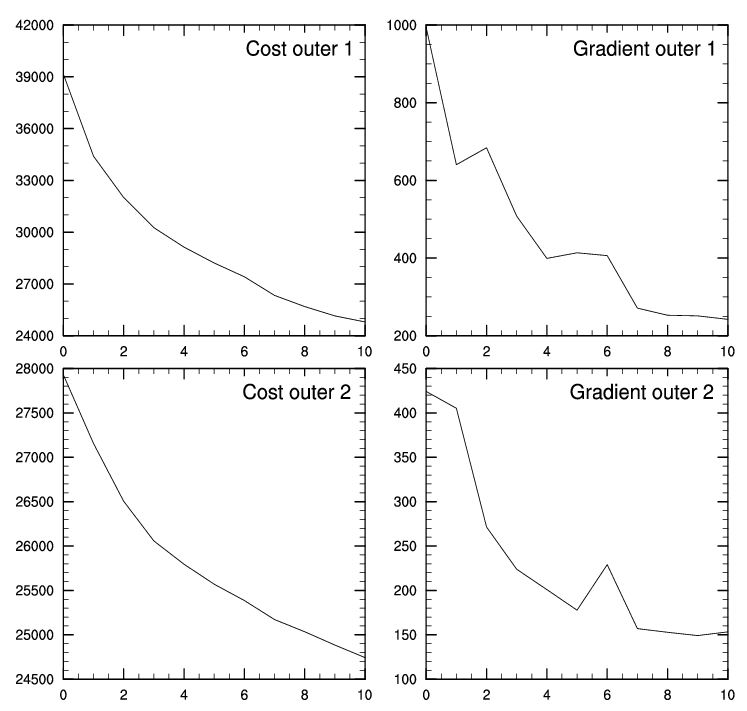
\includegraphics[width=0.7\textwidth]{images/CostGrad}
  \caption{Evolution of the cost function (left column) and the norm of the gradient (right column) in the first outer loop (top row) and the second outer loop (bottom row). The Y-axis is the iteration number.}
  \label{fig:costgrad}
\end{figure}

Scripts are available in the release code to read convergence information from \textit{fort.220} and produce the above plots. Please see Section A.3 for information on where to locate and how to run these scripts.
\end{enumerate}

%-------------------------------------------------------------------------------
\section{Conventional Observation Errors}
%-------------------------------------------------------------------------------

Each observation type has its own observation errors. In this section, we introduce several topics related to the conventional observation error processing in GSI. The observation error for satellite radiance and its adjustment is discussed in the Advanced User\textquotesingle s Guide.

%-------------------------------------------------------------------------------
\subsection{Getting Original Observation Errors}
\label{sec4.7.1}
%-------------------------------------------------------------------------------

For the global GSI analysis, when \verb|oberrflg| (a namelist option in section \verb|&obsqc|) is true, observation errors are generated based on an external observation error table according to the observation type. Otherwise, observation errors are read in from the PrepBUFR file.

For regional analyses, GSI forces the use of an external observation error table to get observation errors no matter what the \verb|oberrflg| is set to (\verb|oberrflg| is forced to be true for regional runs in \textit{gsimod.F90}).

The external observation error table file, \textit{errtable}, includes observation errors for all types of conventional observations. It is copied from the \textit{./fix} directory by the run script. This release package has three sample external observation error table files, \textit{nam\_errtable.r3dv}, \textit{prepobs\_errtable.global}, and \textit{rtma/new\_rtma\_nam\_errtable.r3dv} in the \textit{./fix} directory. The \textit{nam\_errtable.r3dv} is used in the sample run script as a default observation error table. The observation error file is a text file that can be easily edited to tune the error values. The following shows a portion of \textit{nam\_errtable.r3dv} file for rawinsondes and its description of each column in Table \ref{tab410}:

\begin{scriptsize}
\begin{verbatim}
Column # 1         2           3          4           5          6
  120 OBSERVATION TYPE
  0.11000E+04 0.12696E+01 0.60737E+00 0.10000E+10 0.76322E+00 0.10000E+10
  0.10500E+04 0.13282E+01 0.66294E+00 0.10000E+10 0.76322E+00 0.10000E+10
  0.10000E+04 0.13932E+01 0.74223E+00 0.10000E+10 0.76322E+00 0.10000E+10
  0.95000E+03 0.14390E+01 0.83688E+00 0.10000E+10 0.79899E+00 0.10000E+10
  0.90000E+03 0.14354E+01 0.94025E+00 0.10000E+10 0.83561E+00 0.10000E+10
  0.85000E+03 0.13669E+01 0.10439E+01 0.10000E+10 0.87224E+00 0.10000E+10


  220 OBSERVATION TYPE
  0.11000E+04 0.10000E+10 0.10000E+10 0.18521E+01 0.10000E+10 0.10000E+10
  0.10500E+04 0.10000E+10 0.10000E+10 0.20636E+01 0.10000E+10 0.10000E+10
  0.10000E+04 0.10000E+10 0.10000E+10 0.22799E+01 0.10000E+10 0.10000E+10
  0.95000E+03 0.10000E+10 0.10000E+10 0.24211E+01 0.10000E+10 0.10000E+10
  0.90000E+03 0.10000E+10 0.10000E+10 0.24934E+01 0.10000E+10 0.10000E+10
  0.85000E+03 0.10000E+10 0.10000E+10 0.25155E+01 0.10000E+10 0.10000E+10

\end{verbatim}
\end{scriptsize}

\begin{table}[htbp]
\centering
\caption{Description of each column in the observation error table file}
\begin{tabular}{|p{2cm}|p{2cm}|p{2cm}|p{2cm}|p{1cm}|p{1cm}|p{2.5cm}|}
\hline
\hline
 Column \# & 1 & 2 & 3 & 4 & 5 & 6  \\
\hline
\textit{Content} & Pressure & T & RH & UV & Ps & Pw \\
\hline
\textit{Unit} & hPa & degree C & percent/10 & m/s & mb & kg/m2(or mm)\\
\hline
\end{tabular}
\label{tab410}
\end{table} 

For each observation type, the error table has six columns and 33 rows (levels). The 1\textsuperscript{st} column prescribes 33 pressure levels, covering 1100 hPa to 0 hPa. Columns 2-6 prescribe observation errors for temperature (T), relative humidity (RH), horizontal wind component (UV), surface pressure (Ps), and the total column precipitable water (Pw). The missing value is 0.10000E+10. 

The observation error table for each observation type starts with the observation type number defined for the PrepBUFR files, such as:

\begin{scriptsize}
\begin{verbatim}
120 OBSERVATION TYPE
220 OBSERVATION TYPE
\end{verbatim}
\end{scriptsize}

The PrepBUFR data type numbers 100-199 are for temperature (T), moisture (q), and surface pressure (Ps) observations, while numbers 200-299 are for horizontal wind component (UV) observations. A detailed explanation of each data type number can be found in the following table on the EMC website: 

\begin{small}
\url{http://www.emc.ncep.noaa.gov/mmb/data_processing/prepbufr.doc/table_2.htm}
\end{small}

For more details on PrepBUFR/BUFR, please check the BUFR/PrepBUFR User\textquotesingle s Guide, which is freely available at the DTC BUFR/PrepBUFR website:

\begin{small}
\url{http://www.dtcenter.org/com-GSI/BUFR/index.php}
\end{small}

%-------------------------------------------------------------------------------
\subsection{Observation Error Gross Error Check within GSI}
%-------------------------------------------------------------------------------

The gross error check is an important quality control step to exclude questionable observations that degrade the analysis. Users can adjust the threshold of the gross error check for each data type within the \textit{convinfo} file to make the gross error check more or less strict for a certain data type. For example, the following is a part of the \textit{convinfo} file without the last five columns:

\begin{scriptsize}
\begin{verbatim}
!otype  type  sub iuse twindow numgrp ngroup nmiter gross ermax ermin var_b    var_pg ithin
ps       183    0   -1     3.0      0      0      0   4.0   3.0   1.0   4.0  0.000300     0
ps       187    0    1     3.0      0      0      0   4.0   3.0   1.0   4.0  0.000300     0
t        120    0    1     3.0      0      0      0   8.0   5.6   1.3   8.0  0.000001     0
t        126    0   -1     3.0      0      0      0   8.0   5.6   1.3   8.0  0.001000     0
\end{verbatim}
\end{scriptsize}
 
The gross check for each data type is controlled by columns "gross", "ermax", and "ermin." If an observation has observation error set to "obserror," then a gross check ratio is calculated:

\textit{ratio = (Observation-Background)/max(ermin,min(ermax,obserror))}

If \textit{ratio > gross}, then this observation fails the gross check and will not be used in the analysis. The unused observation is indicated as a "rejection" in the fit files.

%-------------------------------------------------------------------------------
\section{Background Error Covariance}
\label{sec4.8}
%-------------------------------------------------------------------------------

The GSI package has several files in \textit{./fix} to hold the pre-computed background error statistics for different GSI applications with different grid configurations. Within the \textit{./fix} subdirectories \textit{./fix/Big\_Endian} and \textit{./fix/Little\_Endian} contain the fix files corresponding to each endianness. Since the GSI code has a build-in mechanism to interpolate the input background error matrix to any desired analysis grid, the following two background error files can be used to specify the B matrix for any GSI regional application.

\begin{itemize}
\item \textit{nam\_nmmstat\_na.gcv} : contains the regional background error statistics, computed using forecasts from the NCEP\textquotesingle s NAM model covering North America. The values of this B matrix cover the northern hemisphere with 93 latitude lines, from -2.5 degrees to 89.5 degrees with 60 vertical sigma levels from 0.9975289 to 0.01364. 
\item \textit{nam\_glb\_berror.f77.gcv} : contains the global background errors based on NCEP\textquotesingle s GFS model, a global forecast model. The values of this B matrix cover the globe with 192 latitude lines from -90 degrees to 90 degrees and 42 vertical sigma levels from 0.99597 to 0.013831.
\end{itemize}

The background error matrix files listed above are in Big Endian binary form (therefore located in the \textit{Big\_Endian} directory). In the \textit{Little\_Endian} directory, \textit{nam\_nmmstat\_na.gcv} and \textit{nam\_glb\_berror.f77.gcv} are their Little Endian versions for certain computer platforms that cannot compile GSI with the Big Endian option. In this release version, GSI can be compiled with the Big Endian option with PGI and Intel.

%-------------------------------------------------------------------------------
\subsection{Tuning Background Error Covariance through the Namelist and Anavinfo File}
%-------------------------------------------------------------------------------

The final background error covariance matrix used in the GSI analysis is the content from the fixed file "berror", which is a copy of \textit{nam\_nmmstat\_na.gcv} or \textit{nam\_glb\_berror.f77.gcv}, multiplied by several factors set by the namelist and the \textbf{anavinfo} file.

In GSI namelist, three variables are used for tuning horizontal and vertical impact scales:

\begin{itemize}
\item \verb|vs|	scale factor for vertical correlation lengths for background error
\item \verb|hzscl(3)| scale factor for three scales specified for horizontal smoothing 
\item \verb|hswgt(3)| weights to apply to each horizontal scales
\end{itemize}

In the GSI anavinfo file, the column \textbf{as/tsfc\_sdv} in the \textit{control\_vector} section are factors for tuning the variance of each analysis control variable.

These values can be used to tune the background error covariance used in the GSI analysis. For each background error matrix file, there are recommended values for these parameters listed in table \ref{tab411}.

\begin{table}[htbp]
\centering
\caption{Recommended tuning values for the provided B matrix.}
\begin{tabular}{|p{2cm}|p{5cm}|p{5cm}|}
\hline
\hline
  & Global & Regional   \\
\hline
\textit{fixed B matrix} & nam\_glb\_berror.f77.gcv & nam\_nmmstat\_na.gcv \\
\hline
\textit{vs} & 0.7 & 1.0\\
\hline
\textit{hzscl} & 1.7, 0.8, 0.5 & 0.373,0.746,1.50\\
\hline
\textit{hswgt} & 0.45, 0.3,0.25 & 0.45, 0.3,0.25\\
\hline
\textit{ss/tsfc\_sdv} & 
\begin{verbatim}
control_vector:: 
!var    as/tsfc_sdv
 sf        0.60
 vp        0.60
 ps        0.75
 t         0.75
 q         0.75
 oz        0.75
 sst       1.00
 cw        1.00
 stl       3.00
 sti       3.00
\end{verbatim}
 & 
\begin{verbatim}
control_vector::
!var    as/tsfc_sdv
 sf        1.00
 vp        1.00
 ps        0.50
 t         0.70
 q         0.70
 oz        0.50
 sst       1.00
 cw        1.00
 stl       1.00
 sti       1.00
\end{verbatim}
\\
\hline
\end{tabular}
\label{tab411}
\end{table} 

%-------------------------------------------------------------------------------
\section{Analysis Increments}
%-------------------------------------------------------------------------------

Analysis increments are defined as the difference between analysis results and the background (A-B). A plot of analysis increments can help users understand how the analysis procedure modifies the background fields according to observations, background and observation error covariances, and other constraints. You can either calculate \textit{analysis-guess} and plot the difference field or use the tools introduced in Appendix A.4 to make analysis increment figures for different analysis fields.

%-------------------------------------------------------------------------------
\section{Running Time and Memory Usage}
%-------------------------------------------------------------------------------

In addition to analysis increments, run time and memory usage are other important features of an analysis system, especially for operational code like the GSI.
 
The GSI standard output file (\textit{stdout}) gives the GSI start time and end time of the analysis at the beginning and end of the file. For example:

\begin{scriptsize}
\begin{verbatim}
* . * . * . * . * . * . * . * . * . * . * . * . * . * . * . * . * . * . * . * .
     PROGRAM GSI_ANL HAS BEGUN. COMPILED 1999232.55     ORG: NP23
     STARTING DATE-TIME  JUL 02,2016  20:36:21.760  184  SAT   2457572

...
 
     ENDING DATE-TIME    JUL 02,2016  20:43:40.422  184  SAT   2457572
     PROGRAM GSI_ANL HAS ENDED.
* . * . * . * . * . * . * . * . * . * . * . * . * . * . * . * . * . * . * . * .
\end{verbatim}
\end{scriptsize}

This tells us the analysis started at 20:36:21.760 and ended at 20:43:40.422, which means GSI used 7 minutes and 19 seconds to finish.

Following the ending date-time, there is a resource statistics section at the end of the \textit{stdout} file, which gives information about run time and memory usage for the analysis:

\begin{scriptsize}
\begin{verbatim}
*****************RESOURCE STATISTICS*******************************
The total amount of wall time                        = 438.663534
The total amount of time in user mode                = 427.578998
The total amount of time in sys mode                 = 9.457562
The maximum resident set size (KB)                   = 2020132
Number of page faults without I/O activity           = 312762
Number of page faults with I/O activity              = 0
Number of times filesystem performed INPUT           = 0
Number of times filesystem performed OUTPUT          = 0
Number of Voluntary Context Switches                 = 7641
Number of InVoluntary Context Switches               = 851
*****************END OF RESOURCE STATISTICS*************************
\end{verbatim}
\end{scriptsize}
